% \setcounter{section}{0}%更改chapter的计数器值
% %\numberwithin{equation}{chapter}%公式计数器从属于节计数器
% \numberwithin{equation}{section}%公式计数器从属于节计数器
% \numberwithin{figure}{section}%图计数器从属于节计数器
% \setcounter{chapter}{5}

%\chapter{\texorpdfstring{树图振幅}{6 Tree-level amplitudes}}
\chapter{树图振幅} \label{cha:6}
我们现在来研究弦相互作用. 在本章, 我们将考察最低阶振幅, 他们来源于欧拉数为正的面, 我们首先描述相关的黎曼面并计算所需要的 CFT 期望值.
接下来我们将研究散射振幅, 首先是开弦, 然后是闭弦. 沿着这条路, 我们在开弦理论中会引入一个重要的推广: Chan-Paton因子. 
在本节末尾我们将回到 CFT, 并讨论期望值的普遍性质.
%\section{\texorpdfstring{Riemann面}{6.1 Riemann surfaces}}

\section{黎曼面} \label{sec:6.1}

欧拉数为正的黎曼面有三种: 球面, 圆盘以及投影平面.

\subsection*{球面}

\begin{figure}
	\begin{center}
		%width=0.8\textwidth,bb=0 0 545 585
		%1px=0.75pt
		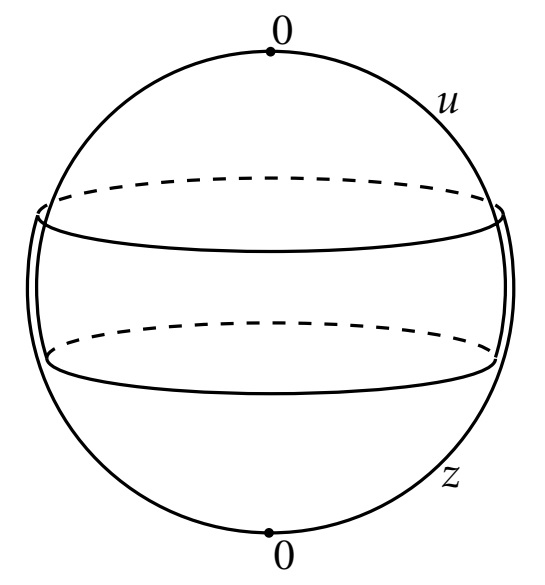
\includegraphics[width=0.5\textwidth,natwidth=408.75,natheight=438.75]{Fig6.1.jpg}\\
		\caption{从$z$坐标卡和$u$坐标卡构建的球面}\label{fig:6.1}
	\end{center}
\end{figure}

球面$S_2$可以被两个坐标卡覆盖, 如图\ref{fig:6.1}所示. 取圆盘$|z|<\rho$ 以及 $|u|<\rho$, 其中 $\rho>1$, 
并通过 
\begin{equation}
u=1 / z  \label{6.1.1}
\end{equation}
来做粘合. 事实上, 我们可以取 $\rho \to \infty$. 这样, 坐标 $z$在``北极''点$u=0$处都是良好的. 

我们可以认为球面是黎曼面, 在两个坐标卡上均取平坦度规, 并用一个共形(坐标加 Weyl)变换连接两个坐标卡. 
或者我们可以将其视为有一个整体定义的度规的黎曼流形. 一般的共形规范度规是
\begin{equation}
	\dif s^{2}=\exp (2 \omega(z, \bar{z})) \dif z \dif \bar{z} \:. \label{6.1.2}
\end{equation}
由于 $\dif z \dif \bar{z}=|z|^{4} \dif u \dif \bar{u}$, 这一度规在$u=0$不奇异的条件是$\exp (2 \omega(z, \bar{z}))$ 在 $z \to \infty $按 $|z|^{-4}$衰减. 例如,
\begin{equation}
	\dif s^{2}=\frac{4 r^{2}\, \dif z \dif \bar{z}}{(1+z \bar{z})^{2}}=\frac{4 r^{2}\, \dif u \dif \bar{u}}{(1+u \bar{u})^{2}} \label{6.1.3}
\end{equation}
描述了半径为 $r$, 曲率为 $R=2 / r^{2}$的球面.

根据\ref{sec:5.2}节的普遍讨论, 球面没有模但有6个CKV, 使得每个度规 (diff $\times$ Weyl)等价于\eqref{6.1.3}. 
我们在无限小层次观察这一点. 正如在\eqref{5.2.8}寻找的是全纯张量场$\delta g_{z z}(z)$ 和全纯矢量场 $\delta z(z)$. 
这些必须定义在整个球面上, 所以我们要考察到$u$坐标卡的变换
\begin{subequations}  \label{6.1.4}
	\begin{align}
		\delta u &=\frac{\partial u}{\partial z} \delta z=-z^{-2} \delta z \:, \label{6.1.4a} \\
		\delta g_{u u} &=\left(\frac{\partial u}{\partial z}\right)^{-2} \delta g_{z z}=z^{4} \delta g_{z z} \:. \label{6.1.4b} 
	\end{align}
\end{subequations}
任何全纯二次微分 $\delta g_{z z}$ 必须关于 $z$ 全纯, 并且在无穷远处以 $z^{-4}$ 趋于零, 因而必须恒等于零. 
另一方面, $\mathrm{CKV} \delta z$在 $u=0$全纯使得它在 $z \rightarrow \infty$增长不超过 $z^{2}$. 那么一般的 $\mathrm{CKV}$ 是
\begin{subequations} \label{6.1.5}
	\begin{align}
		\delta z       &= a_{0}+a_{1} z+a_{2} z^{2}  \:, \label{6.1.5a} \\
		\delta \bar{z} &= a_{0}^{*}+a_{1}^{*} \bar{z}+a_{2}^{*} \bar{z}^{2} \:, \label{6.1.5b}
	\end{align}
\end{subequations}
其有3个复参量或6个实参量, 正是黎曼-罗赫定理所期待的.


这些无限小变换指数化就给出了 \emph{M\"{o}bius 群}
\begin{equation}
	z^{\prime}=\frac{\alpha z+\beta}{\gamma z+\delta} \:. \label{6.1.6}
\end{equation}
重新调整 $\alpha, \beta, \gamma, \delta $ 不会使得变换改变, 所以我们可以固定 $\alpha \delta-\beta \gamma=1$并在 $\alpha, \beta, \gamma, \delta $ 的全部负号反演下等价, 这定义了 $P S L(2, \mathds{C})$群. 这是在整个$S_{2}$上全纯的最普遍的坐标变换. 它是含有无穷远点的一一映射. 
6个参量中的3个对应普通旋转, 构成 $PSL(2, \mathds{C})$的子群$SO(3)$. 

\subsection*{圆盘}

在反射下将球面上的两个点等价, 可以从球面构建出圆盘$D_{2}$. 例如, 等价 $z$ 和 $z^{\prime}$ 使得
\begin{equation}
	z^{\prime}=1 / \bar{z} \:. \label{6.1.7}
\end{equation}
在极坐标$z=r \me^{\mi \phi}$下, 这对半径求倒数, 但保持角度, 所以单位圆盘$|z| \leq 1$是粘合后的基本域. 单位圆上的点被反射所固定, 所以它变成一个边界. 
使用共形等价反演
\begin{equation}
	z^{\prime}=\bar{z}  \label{6.1.8}
\end{equation}
通常会方便些. 现在上半平面是基本域, 而实轴是边界.

圆盘的 CKG 是$PSL(2, \mathds{C})$的子群, 该子群保持圆盘的边界不变. 
对于反演\eqref{6.1.8}, 这就是\eqref{6.1.6}中 $\alpha, \beta, \gamma, \delta$ 全为实数的子群, 即 $P S L(2, \mathds{R})$, 实参量的 Möbius 群. 
一个 CKV 是圆盘上的普通旋转对称性. 又一次, 所有度规都等价, 不存在模.

\subsection*{射影平面}

射影平面$R P_{2}$ 也可以作为球面的 $\mathds{Z}_{2}$粘合获得. 将
\begin{equation}
	z^{\prime}=-1 / \bar{z} \label{6.1.9}
\end{equation}
的两个点 $z$ 和$z^{\prime}$粘合起来. 这些点在圆度规\eqref{6.1.3}中是对径点. 不存在固定点, 所以在相应空间中没有边界, 但这个空间是非定向的. 
该粘合的一个基本域是单位圆盘 $|z| \leq 1$, 不过点 $\me^{\mi \phi}$ 与 $-\me^{\mi \phi}$ 被粘合. 
另一选择是上半$z$平面, 不存在模. CKG 是反映\eqref{6.1.9}粘合的 $P S L(2, \mathds{C})$ 的子群; 这就是普通的旋转群 $SO(3)$.

圆盘和射影平面都可以表示为球面, 其上的点在$\mathds{Z}_{2}$ 变换或\emph{乘方(involution)}下粘合. 
事实上, 每一个世界面都可以在一个或两个 $\mathds{Z}_{2} $下粘合, 从闭的定向曲面下获得. 这样, 就可用镜像法获取 格林 函数.

\section{标量的期望值} \label{sec:6.2}

我们所需要的基本量是顶点算符的期望值. 为了发展几个有用的技巧和观点, 我们将以三种不同的方式计算它们: 直接的路径积分、使用全纯性, 以及本章后面的算符方法.

路径积分方法已经用于\ref{sec:5.3}节Faddeev-Popov行列式以及附录中的谐振子. 从一般泛函出发: 
\begin{equation}
	Z[J]=\left\langle\exp \left(\mi \int \dif^{2} \sigma\: J(\sigma) \cdot X(\sigma)\right)\right\rangle \label{6.2.1}
\end{equation}
其中 $J_{\mu}(\sigma) $任意. 从现在起, 我们在任意的紧致二维平面 $M$上进行处理, 时空维数是$d$. 
在完备基 $\mathsf{X}_{I}(\sigma)$上展开$X^{\mu}(\sigma)$ 
\begin{subequations} \label{6.2.2}
\begin{align}
X^{\mu}(\sigma) &= \sum_{I} x_{I}^{\mu} \mathsf{X}_{I}(\sigma) \:, \label{6.2.2a} \\
\nabla^{2} \mathsf{X}_{I} &= -\omega_{I}^{2} \mathsf{X}_{I} \:,  \label{6.2.2b} \\
\int_{M} \dif^{2} \sigma\: g^{1 / 2} \mathsf{X}_{I} \mathsf{X}_{I^{\prime}} &= \delta_{I I^{\prime}} \:.  \label{6.2.2c} 
\end{align}	
\end{subequations}
那么
\begin{equation}
	Z[J]=\prod_{I, \mu} \int \dif x_{I}^{\mu} \exp \left(-\frac{\omega_{I}^{2} x_{I}^{\mu} x_{I \mu}}{4 \pi \alpha^{\prime}}+\mi x_{I}^{\mu} J_{I \mu}\right) \:, \label{6.2.3}
\end{equation}
其中
\begin{equation}
	J_{I}^{\mu}=\int \dif^{2} \sigma J^{\mu}(\sigma) \mathsf{X}_{I}(\sigma) \:. \label{6.2.4}
\end{equation}


除了常模
\begin{equation}
	\mathsf{X}_{0}=\left(\int \dif^{2} \sigma \: g^{1 / 2}\right)^{-1 / 2} \:, \label{6.2.5}
\end{equation}
这个积分是高斯型的. 常模的作用量为零, 所以给出$\delta$-函数. 
\begin{tcolorbox}
	\begin{remark}
		对于$I=0$, \eqref{6.2.3}给出
		\[
			\int \dif x^{\mu}_{0} \: \exp (\mi x^{\mu}_{0}J_{0\mu}) \propto \delta^{d}(J_{0}) \:.
		\]
	\end{remark}
\end{tcolorbox}
\noindent 算出积分得到
	\begin{align}
		Z[J] &= \mi(2 \pi)^{d} \delta^{d}(J_{0}) \prod_{I \neq 0} \left(\frac{4 \pi^{2} \alpha^{\prime}}{\omega_{I}^{2}}\right)^{d / 2} \exp \left(-\frac{\pi \alpha^{\prime} J_{I} \cdot J_{I}}{\omega_{I}^{2}}\right) \nonumber  \\
		&= \mi(2 \pi)^{d} \delta^{d}\left(J_{0}\right)\left(\operatorname{det}^{\prime} \frac{-\nabla^{2}}{4 \pi^{2} \alpha^{\prime}}\right)^{-d / 2} \nonumber  \\
		& \qquad \quad \times \exp \left(-\frac{1}{2} \int \dif^{2} \sigma \, \dif^{2} \sigma^{\prime}\: J(\sigma) \cdot J(\sigma^{\prime}) 
		G^{\prime}(\sigma, \sigma^{\prime})\right) \:. \label{6.2.6}
	\end{align}
正如\ref{sec:2.1}节和\ref{sec:3.2}节讨论的, 类时模 $x_{I}^{0}$ 产生的Gauss积分符号是错的, 因此通过围道转动定义$x_{I}^{0} \to-\mi x_{I}^{d}, I \neq 0 $.\footnote{$\mi$是手加的, 因为我们并不想旋转$x_0^0$, 为了得到能量$\delta$函数要转回来} 加撇的格林函数去掉了零模贡献
\begin{equation}
	G^{\prime}(\sigma_{1}, \sigma_{2})=\sum_{I \neq 0} \frac{2 \pi \alpha^{\prime}}{\omega_{I}^{2}} \mathsf{X}_{I}(\sigma_{1}) \mathsf{X}_{I}(\sigma_{2}) \:. \label{6.2.7}
\end{equation}
它满足微分方程
	\begin{align}
		-\frac{1}{2 \pi \alpha^{\prime}} \nabla^{2} G^{\prime}(\sigma_{1}, \sigma_{2}) 
		&=\sum_{I \neq 0} \mathsf{X}_{I}(\sigma_{1}) \mathsf{X}_{I}(\sigma_{2})  \nonumber \\
		&=g^{-1 / 2} \delta^{2}(\sigma_{1}-\sigma_{2})-\mathsf{X}_{0}^{2}  \:, \label{6.2.8}
	\end{align}
其中使用了 $\mathsf{X}_{I}$ 的完备性. 那种源为$\delta$-函数的普通 格林 函数不存在. 它会对应单个电荷的静电势, 但在紧致面上, 从源流出的场线没有地方可去. 
$\mathsf{X}_{0}^{2}$项可视为用来中和的背景电荷分布.


\subsection*{球面}
具体到球面上, 微分方程\eqref{6.2.8}的解是
\begin{equation}
	G^{\prime}(\sigma_{1}, \sigma_{2})=-\frac{\alpha^{\prime}}{2} \ln |z_{12}|^{2}+f(z_{1}, \bar{z}_{1})+f(z_{2}, \bar{z}_{2}) \:, \label{6.2.9}
\end{equation}
\begin{tcolorbox}
	\begin{remark}
		在球面上$g=\me^{4 \omega}$, $\nabla^{2}=\me^{-2 \omega} \partial \bar{\partial}$, 那么\eqref{6.2.8}变成
		\[
		\partial \bar{\partial} G^{\prime}=-2 \pi \alpha^{\prime} \delta^{2}(\sigma_{1}-\sigma_{2})
		+2 \pi \alpha^{\prime} \me^{2 \omega}\,\mathsf{X}_{0}^{2} 
		\]
		而$
		\partial \bar{\partial} \ln |z_{12}|^{2}=2 \pi \delta^{2}(z, \bar{z})=4 \pi \delta^{2}(\sigma_{1}-\sigma_{2})
		$.
		\end{remark}
\end{tcolorbox}
\noindent 其中
\begin{equation}
	f(z, \bar{z})=\frac{\alpha^{\prime} \mathsf{X}_{0}^{2}}{4} 
	\int \dif^{2} z^{\prime}\: \exp [2 \omega(z^{\prime}, \bar{z}^{\prime})] \ln|z-z^{\prime}|^{2}+k \:. \label{6.2.10}
\end{equation}
$G^{\prime}$ 与 $\mathsf{X}_{0}$正交的性质决定常数$k$, 但在任何情况下, 我们将看到函数$f$与所有期望值无关. 
它来源于背景电荷, 但来自零模积分的$\delta$-函数迫使整体中性,  $J_{0}^{\mu}=0$, 而背景场没有净贡献.

现在考察含有快子顶点算符乘积的路径积分
\begin{equation}
	A_{S_{2}}^{n}(k, \sigma)=\left\langle\left[\me^{\mi k_{1} \cdot X(\sigma_{1})}\right]_{\mathrm{r}}
	\left[\me^{\mi k_{2} \cdot X(\sigma_{2})}\right]_{\mathrm{r}} \cdots
	\left[\me^{\mi k_{n} \cdot X(\sigma_{n})}\right]_{\mathrm{r}}\right\rangle_{S_{2}} \:. \label{6.2.11}
\end{equation}
这对应于
\begin{equation}
	J(\sigma)=\sum_{i=1}^{n} k_{i} \delta^{2}(\sigma-\sigma_{i}) \:. \label{6.2.12}
\end{equation}
那么振幅\eqref{6.2.6}变成
	\begin{align}
		A_{S_{2}}^{n}(k, \sigma) &=\mi C_{S_{2}}^{X}(2 \pi)^{d} \delta^{d}({\textstyle \sum_{i}} k_{i}) \nonumber \\
		& \quad \times \exp \Biggl(-\sum_{ i<j}^{n} k_{i} \cdot k_{j} G^{\prime}(\sigma_{i}, \sigma_{j})
		-\frac{1}{2} \sum_{i=1}^{n} k_{i}^{2} G_{\mathrm{r}}^{\prime}(\sigma_{i}, \sigma_{i})\Biggr) \:. \label{6.2.13}
	\end{align}
这里的常数是
\begin{equation}
	C_{S_{2}}^{X}=\mathsf{X}_{0}^{-d}\left(\operatorname{det}^{\prime} \frac{-\nabla^{2}}{4 \pi^{2} \alpha^{\prime}}\right)_{S_{2}}^{-d/2} 
	\:. \label{6.2.14}
\end{equation}
\begin{tcolorbox}
	\begin{remark}
		根据\eqref{6.2.4}和\eqref{6.2.5}, $J_{0}=\int \dif^{2} \sigma \: \mathsf{X}_{0} J(\sigma)= \mathsf{X}_{0} \sum_{i} k_{i} $, 
		那么$\delta^{d}(J_{0})=\mathsf{X}_{0}^{-d} \delta^{d}(\sum_{i} k_{i})$.
	\end{remark}
\end{tcolorbox}
\noindent 行列式可以被正规化并计算出来, 但我们不需要显式地计算. 我们在这里采用\ref{sec:3.6}节中的重整化, 使得自收缩包含
\begin{equation}
	G_{\mathrm{r}}^{\prime}(\sigma, \sigma^{\prime})=G^{\prime}(\sigma, \sigma^{\prime})
	+\frac{\alpha^{\prime}}{2} \ln d^{2}(\sigma, \sigma^{\prime}) \:. \label{6.2.15}
\end{equation}
注意到
\begin{equation}
	G_{\mathrm{r}}^{\prime}(\sigma, \sigma)=2 f(z, \bar{z})+\alpha^{\prime} \omega(z, \bar{z}) \label{6.2.16}
\end{equation}
是有限的. 
那么球面上的路径积分是
\begin{equation}
	A_{S_{2}}^{n}(k, \sigma)=\mi C_{S_{2}}^{X}(2 \pi)^{d} \delta^{d}({\textstyle \sum_{i}} k_{i}) 
	\exp \left(-\frac{\alpha^{\prime}}{2} \sum_{i} k_{i}^{2} \omega\left(\sigma_{i}\right)\right) 
	\prod_{i<j}|z_{i j}|^{\alpha^{\prime} k_{i} \cdot k_{j}} \:. \label{6.2.17}
\end{equation}
对共形因子 $\omega(\sigma)$的依赖关系是从顶点算符的Weyl反常中获得的. 对于在壳算符它将抵消 $g^{1 / 2}$ 的变分.我们会在一个很大的包含所有顶点算符的区域内取度规为平坦(将曲率推向无穷大), 那么$\omega(\sigma_{i})$中的项就被扔掉了.
\begin{tcolorbox}
	关于\eqref{6.2.16}的注解:
	\[
		\ln d^{2}(\sigma, \sigma^{\prime})-\ln |z_{12}|^{2}=
		\ln \left(\frac{\int \me^{2 \omega} \: \dif z \dif \bar{z}}{\int \dif z \dif  \bar{z}}\right)=2 \omega	
	\]
	关于\eqref{6.2.17}的注解: 以$n=2$为例, 依赖$f$的部分是 
\[
k_{1} k_{2} (f_{1}+f_{2})+\frac{1}{2} k_{1}^{2} \cdot 2 f_{1}+\frac{1}{2} k_{2}^{2} \cdot 2 f_{2} 
=(k_{1} f_{1}+k_{2} f_{2})(k_{1}+k_{2})
\]
由于路径积分中含有$\delta(\sum_{i} k_{i})= k_{1}+k_{2}$, 所以它与$f$无关.
\end{tcolorbox}

高阶顶点算符是e指数乘以$X^{\mu}$的偏导, 所以我们又需要
\begin{equation}
	\Biggl\langle\prod_{i=1}^{n}\left[\me^{\mi k_{i} \cdot X(z_{i}, \bar{z}_{i})}\right]_{\mathrm{r}} 
	\prod_{j=1}^{p} \partial X^{\mu_{j}}(z_{j}^{\prime}) \prod_{k=1}^{q} \bar{\partial} X^{\nu_{k}}(\bar{z}_{k}^{\prime \prime})\Biggr\rangle \biggr._{\!\!S_{2}} \:. \label{6.2.18}
\end{equation}
这由对所有的收缩求和给出, 其中每一个 $\partial X$ 或 $\bar{\partial} X$ 必须要与一个指数或其他 $\partial X$ 和 $\bar{\partial} X$收缩. 
$XX$收缩就是 $-\frac{1}{2} \alpha^{\prime} \ln |z|^{2}$, $f$又一次在最终表达式中扔掉了. 这一结果总结为
	\begin{align}
		&\mi C_{S_{2}}^{X}(2 \pi)  \delta^{d}({\textstyle\sum_{i} }k_{i}) 
		\exp\Biggl(-\frac{\alpha'}{2}\sum_{i}k_{i}^{2}\omega(\sigma_{i})\Biggr)
		\prod_{i<j}^{n}|z_{i j}|^{\alpha^{\prime} k_{i} \cdot k_{j}}  \nonumber \\
		& \qquad \quad \times\Biggl\langle 
		\prod_{j=1}^{p}\Bigl[v^{\mu_{j}}(z_{j}^{\prime})+q^{\mu_{j}}(z_{j}^{\prime})\Bigr] 
		\prod_{k=1}^{q}\Bigl[\tilde{v}^{\nu_{k}}(\bar{z}_{k}^{\prime \prime})+\tilde{q}^{\nu_{k}}(\bar{z}_{k}^{\prime \prime})\Bigr]\Biggr\rangle  \label{6.2.19}
	\end{align}
这里
\begin{equation}
	v^{\mu}(z)=- \mi \frac{\alpha^{\prime}}{2} \sum_{i=1}^{n} \frac{k_{i}^{\mu}}{z-z_{i}}, \qquad 
	\tilde{v}^{\mu}(\bar{z})=-\mi \frac{\alpha^{\prime}}{2} \sum_{i=1}^{n} \frac{k_{i}^{\mu}}{\bar{z}-\bar{z}_{i}} \label{6.2.20}
\end{equation}
来源于与指数的收缩. $q^{\mu}=\partial X^{\mu}-v^{\mu}$的期望值利用$-\eta^{\mu \nu}(z-z^{\prime})^{-2} \alpha^{\prime} / 2$收缩并求和给出, 
而$\tilde{q}^{\nu}$的期望值通过共轭给出.

现在我们以一个不同的方式重新计算, 利用全纯性. 作为一个例子, 考察
\begin{equation}
	\langle\partial X^{\mu}(z_{1}) \partial X^{\nu}(z_{2})\rangle_{S_{2}} \:. \label{6.2.21}
\end{equation}
OPE 决定了它是
\begin{equation}
	-\frac{\alpha^{\prime} \eta^{\mu \nu}}{2 z_{12}^{2}}\langle 1\rangle_{S_{2}}+g(z_{1}, z_{2}) \:, \label{6.2.22}
\end{equation}
其中$g(z_{1}, z_{2})$ 关于两个变量都是全纯的. 在$u$坐标卡,
\begin{equation}
	\partial_{u} X^{\mu}=-z^{2} \partial_{z} X^{\mu} \:, \label{6.2.23}
\end{equation}
所以, 在$u=0$处的全纯性条件就是 $\partial_{z} X^{\mu}$ 的期望值在$z$趋于无穷时像 $z^{-2}$ 那样衰减. 
更一般地, 权重为 $(h, 0)$ 的张量在无穷处的行为是 $z^{-2 h}$. 专注于\eqref{6.2.22}在固定的 $z_{2}$ 处对 $z_{1}$的相关性, 
这暗示 $g(z_{1}, z_{2})$ 在无穷远处像 $z_{1}^{-2}$ 那样衰减, 因而因子全纯性为零. 与路径积分结果\eqref{6.2.19}相比, 这是一致的. 
尽管 $\langle 1\rangle_{S_{2}}$ 看起来像 $\delta(0) $那样发散. 这只是来自无限时空体积的零模发散.

至于顶点算符乘积的期望值
\begin{equation}
	A_{S_{2}}^{n}(k, \sigma)=\left\langle\prod_{i=1}^{n}:\mathrel{\me^{\mi k_{i} \cdot X(z_{i}, \bar{z}_{i})}}:\right\rangle \Big._{\!S_{2}}
	\label{6.2.24}
\end{equation}
用这一方法计算就不那么直接, 这是因为它们不是全纯的. 实际上, 它们因式分解出全纯和反全纯部分, 但这很微妙, 最好用算符的语言引入, 我们会在第\ref{cha:8}章做这件事. 
我们使用平移流的全纯性. 考察附加一个流 $\partial X^{\mu}(z)$的期望值. 流与顶点算符的 OPE 决定$z$的奇异性
\begin{equation}
		\left\langle\partial X^{\mu}(z) \prod_{i=1}^{n}:\mathrel{\me^{\mi k_{i} \cdot X(z_{i}, \bar{z}_{i})}}:\right
		\rangle\bigg._{\!S_{2}}=-\frac{\mi \alpha^{\prime}}{2} A_{S_{2}}^{n}(k, \sigma) \sum_{i=1}^{n} \frac{k_{i}^{\mu}}{z-z_{i}} 
		+\text{在$z$处全纯的项} \:. \label{6.2.25}
\end{equation}
现观察 $z \rightarrow \infty$.  $\partial_{u} X^{\mu}$ 在$u=0$ 处全纯这个条件又一次要求这个期望值在 $z \rightarrow \infty$像 $z^{-2}$ 那样趋于零. 
那么\eqref{6.2.25}的全纯项为零, 并且从 $z^{-1}$阶项为零. 我们发现了动量守恒
\begin{equation}
	A_{S_{2}}^{n}(k, \sigma) \sum_{i=1}^{n} k_{i}^{\mu}=0 \:. \label{6.2.26}
\end{equation}
我们以稍微不同的方式说明它. 考察时空平移流的围道积分
\begin{equation}
	p^{\mu}=\frac{1}{2 \pi \mi} \oint_{C}(\dif z \: j_{z}^{\mu}-\dif \bar{z}\: j_{\bar{z}}^{\mu}) \:, \label{6.2.27}
\end{equation}
其中围道 $C$ 将所有指数算符包含在内. 有两种方法计算它. 
其一是收缩围道$C$, 直到它围绕每个顶点算符变成小圆, 这从每个 OPE 中挑出 $(z-z_{i})^{-1}$ 项, 并给出$\sum_{i=1}^{n} k_{i}^{\mu} $. 
其二是将其扩张, 直到它在$u$坐标卡上是个小圆: 由于在 $u=0$处的全纯性, 它必须为零. 这种变形围道的讨论在 CFT 中广泛使用. 

我们已经使用 OPE 决定奇异性, 然后用全纯性完全觉得了如何依赖$z$. 现在我们来看一下在$z \rightarrow z_{1}$时 OPE 的第二项. 
展开\eqref{6.2.25}给出
\begin{equation}
	-\frac{\mi \alpha^{\prime}}{2} A_{S_{2}}^{n}(k, \sigma)\left(\frac{k_{1}^{\mu}}{z-z_{1}}+\sum_{i=2}^{n} \frac{k_{i}^{\mu}}{z_{1}-z_{i}}+O(z-z_{1})\right) \:. \label{6.2.28}
\end{equation}
与 $\mi k_{1}^{\mu}$收缩,  $(z-z_{1})^{0}$ 阶项必须与 OPE 一致
	\begin{align}
		\mi k_{1} \cdot \partial X(z): \mathrel{\me^{\mi k_{1} \cdot X(z_{1}, \bar{z}_{1})}}: =\frac{\alpha^{\prime} k_{1}^{2}}{2(z-z_{1})} :\mathrel{\me^{\mi k_{1} \cdot X(z_{1}, \bar{z}_{1})}}:
		+ \: \partial_{z_{1}}{:\mathrel{\me^{\mi k_{1} \cdot X(z_{1}, \bar{z}_{1})}}:}+ O(z-z_{1}) \:. \label{6.2.29}
	\end{align}
这暗示了
\begin{equation}
	\partial_{z_{1}} A_{S_{2}}^{n}(k, \sigma)=\frac{\alpha^{\prime}}{2} A_{S_{2}}^{n}(k, \sigma) \sum_{i=2}^{n} \frac{k_{1} \cdot k_{i}}{z_{1 i}} \:. \label{6.2.30}
\end{equation}
积分, 并使用共轭方程以及动量守恒. 在相差归一化的意义下, 这决定了路径积分
\begin{equation}
	A_{S_{2}}^{n}(k, \sigma) \propto \delta^{d}({\textstyle \sum_{i} k_{i}}) 
	\prod_{i<j}^{n} |z_{i j}|^{\alpha^{\prime} k_{i} \cdot k_{j}} \:, \label{6.2.31}
\end{equation}
这与第一种方法一致.注意到为了比较, 我们必须将曲率推向无穷大$(\omega(\sigma_{i})=0)$, 这使得$[]_{\mathrm{r}}=::$.

值得注意的是, 在路径方法的中间步骤中, 依赖于黎曼度规的特定选择. 需要这个度规是为了保护这些步骤中的坐标不变性. 
两个不同的度规, 若 Weyl 等价, 却给出不同的拉普拉斯算符和本征函数. 但在最后, 在弦论中, 这些相关性必须被扔掉. 
第二种方法仅使用黎曼面的基本性质, 它的全纯性.


\subsection*{圆盘}

到圆盘的推广是直接的. 通过取上面球面的表示并将$z$约束至上半复平面, 我们得到圆盘的表示. Neumann 边界项解释为镜像荷
\begin{equation}
	G^{\prime}(\sigma_{1}, \sigma_{2})=-\frac{\alpha^{\prime}}{2} \ln |z_{1}-z_{2}|^{2}
	-\frac{\alpha^{\prime}}{2} \ln |z_{1}-\bar{z}_{2}|^{2} \:, \label{6.2.32}
\end{equation}
会相差一个由于动量守恒而被扔掉的项. 那么
	\begin{align}
		\left\langle\prod_{i=1}^{n}: \mathrel{\me^{\mi k_{i} \cdot X(z_{i}, \bar{z}_{i})}}:\right\rangle \bigg._{\!\!D_{2}} 
		=& \mi C_{D_{2}}^{X} (2 \pi)^{d} \delta^{d}({\textstyle\sum_{i} k_{i}}) 
		\prod_{i=1}^{n}|z_{i}-\bar{z}_{i}|^{\alpha^{\prime} k_{i}^{2} / 2}  \nonumber \\
		& \times \prod_{ i<j}^{n} |z_{i}-z_{j}|^{\alpha^{\prime} k_{i} \cdot k_{j} }
		|z_{i}-\bar{z}_{j}|^{\alpha^{\prime} k_{i} \cdot k_{j}} \:. \label{6.2.33}
	\end{align}
对于含有$\partial_{a} X^{\mu}$ 的期望值, 要再一次对收缩求和, 不过现在使用格林函数\eqref{6.2.32}. 
注意到 $\partial X^{\mu}(z) \bar{\partial} X^{\nu}(\bar{z}^{\prime})$ (或者$ q^{\mu}(z) \tilde{q}^{\nu}(\bar{z}^{\prime})$) 有一个非零的收缩.

对于边界上的两点, 格林函数\eqref{6.2.32}中的两项是相等的, 即便在正规编序减掉第一项后, 格林函数依旧在零间隔处发散. 
由于这个原因, 边界算符必须用边界正规编序(boundary normal ordering)定义, 其中减除(subtraction)加倍了:
\begin{equation}
	 \bno X^{\mu}(y_{1}) X^{\nu}(y_{2})\bno = X^{\mu}(y_{1}) X^{\nu}(y_{2})+2 \alpha^{\prime} \eta^{\mu \nu} 
	 \ln |y_{1}-y_{2}| \:,  \label{6.2.34}
\end{equation}
其中$y$代表实轴上的坐标. 组合学(combinatorics)与其他形式的正规序相同. 边界算符的边界正规编序期望值与内部的共形正规序算符由同样良好的性质 (没有奇异性).

若一个期望值既含有边界上的指数, 又含有内部的指数, 每一个都含有合适的正规编序, 
对于边界算符扔掉 $|z_{i}-\bar{z}_{i}|^{\alpha^{\prime} k_{i}^{2} / 2}$ 因子并对内部结果\eqref{6.2.33}取恰当极限. 
显式地, 对于都在边界上的指数,
\begin{equation}
	\left\langle\prod_{i=1}^{n} \bno \me^{\mi k_{i} \cdot X(y_{i})} \bno \right\rangle\bigg._{\!\!D_{2}}
	=\mi C_{D_{2}}^{X}(2 \pi)^{d} \delta^{d}(\textstyle{\sum_{i} k_{i}} ) 
	\prod_{i<j}^{n}|y_{i}-y_{j}|^{2 \alpha^{\prime} k_{i} \cdot k_{j}} \:. \label{6.2.35}
\end{equation}
更一般地,
\begin{align}
& \left\langle\prod_{i=1}^{n} \bno \me^{\mi k_{i} \cdot X(y_{i})} \bno 
\prod_{j=1}^{p} \partial_{y}X^{\mu_{j}}(y_{j}^{\prime})\right\rangle\bigg._{\!\!D_{2}}
= \mi C_{D_{2}}^{X}(2 \pi)^{d} \delta^{d}({\textstyle \sum_{i} k_{i}})  \nonumber \\
&\qquad \qquad \qquad \qquad  \times \prod_{i<j}^{n}|y_{i j}|^{2 \alpha^{\prime} k_{i} \cdot k_{j}}
\left\langle\prod_{j=1}^{p}\Bigl[v^{\mu_{j}}(y_{j}^{\prime})+q^{\mu_{j}}(y_{j}^{\prime})\Bigr]\right\rangle\bigg._{\!\! D_{2}} \:, 
\label{6.2.36}
\end{align}
其中
\begin{equation}
	v^{\mu}(y)=-2 \mi \alpha^{\prime} \sum_{i=1}^{n} \frac{k_{i}^{\mu}}{y-y_{i}} \label{6.2.37}
\end{equation}
而$q$用$-2 \alpha^{\prime}(y-y^{\prime})^{-2} \eta^{\mu \nu}$收缩.

\subsection*{射影平面}
镜像法给出的格林函数是
\begin{equation}
	G^{\prime}(\sigma_{1}, \sigma_{2})=-\frac{\alpha^{\prime}}{2} \ln |z_{1}-z_{2}|^{2}
	-\frac{\alpha^{\prime}}{2} \ln |1+z_{1} \bar{z}_{2}|^{2} \:. \label{6.2.38}
\end{equation}
现在
	\begin{align}
		\left\langle\prod_{i=1}^{n}:\mathrel{\me^{\mi k_{i} X(z_{i}, \bar{z}_{i})}}:\right\rangle\bigg._{\!\! RP_{2}} 
		&=\mi C_{RP_{2}}^{X}(2 \pi)^{d} \delta^{d}({\textstyle\sum_{i} k_{i}}) 
		\prod_{i=1}^{n}|1+z_{i} \bar{z}_{i}|^{\alpha^{\prime} k_{i}^{2} / 2} \nonumber \\
		&\quad  \times \prod_{i<j}^{n}|z_{i}-z_{j}|^{\alpha^{\prime} k_{i} \cdot k_{j}}|1+z_{i} \bar{z}_{j}|^{\alpha^{\prime} k_{i} k_{j}} \:, \label{6.2.39}
	\end{align}
对于更一般的期望值以此类推. 由于不包含固定点, 点$z$不可能接触到它的像 $-\bar{z}^{-1}$, 所以不存在边界.

\newpage

\section{\texorpdfstring{$bc$共形场论}{bc共形场论}} \label{sec:6.3}

\subsection*{球面}

鬼场的路径积分已经在\ref{sec:5.3}节建立. 根据黎曼—罗赫定理, 最简单且非零的期望值是
\begin{equation}
	\langle c(z_{1}) c(z_{2}) c(z_{3}) \tilde{c}(\bar{z}_{4}) \tilde{c}(\bar{z}_{5}) \tilde{c}(\bar{z}_{6})\rangle_{S_{2}} \:. \label{6.3.1}
\end{equation}
相差一个归一化(即, 一个泛函行列式)的意义下, 结果\eqref{5.3.18}就是零模行列式
\begin{equation}
	\operatorname{det} \mathsf{C}_{0 j}^{a}(\sigma_{i}) \:. \label{6.3.2}
\end{equation}
在\ref{sec:6.1}节找到6个 CKV. 在复基下, 它们是
\begin{subequations} \label{6.3.3}
\begin{align}
\mathsf{C}^{z} &= 1, z, z^{2}\:, \quad \mathsf{C}^{\bar{z}}=0  \:, \label{6.3.3a} \\
\mathsf{C}^{z} &= 0\:, \quad \mathsf{C}^{\bar{z}}=1, \bar{z}, \bar{z}^{2} \:. \label{6.3.3b}
\end{align}
\end{subequations}
在这一基下, 行列式分裂成了两个 $3 \times 3$ 块, 而期望值变成
\begin{equation}
	C_{S_{2}}^{\mathrm{g}} \operatorname{det}\left|\begin{array}{ccc}
		1 & 1 & 1 \\
		z_{1} & z_{2} & z_{3} \\
		z_{1}^{2} & z_{2}^{2} & z_{3}^{2}
	\end{array}\right| \operatorname{det}\left|\begin{array}{ccc}
		1 & 1 & 1 \\
		\bar{z}_{4} & \bar{z}_{5} & \bar{z}_{6} \\
		\bar{z}_{4}^{2} & \bar{z}_{5}^{2} & \bar{z}_{6}^{2}
	\end{array}\right|=C_{S_{2}}^{\mathrm{g}} z_{12} z_{13} z_{23} \bar{z}_{45} \bar{z}_{46} \bar{z}_{56} \:. \label{6.3.4}
\end{equation}
常数$C_{S_{2}}^{\mathrm{g}}$ 包含泛函行列式以及有限维雅可比行列式(独立于位置), 产生雅可比行列式是因为基\eqref{6.3.3}不是正交的. 

对于树图振幅, 这是我们唯一需要的$b c$路径积分, 但完整期见, 我们给出
\begin{align}
\left\langle\prod_{i=1}^{p+3} c(z_{i}) \prod_{j=1}^{p} b(z_{j}^{\prime}) \cdot(\text{反全纯})\right\rangle\bigg._{\!\!S_{2}}
&=C_{S_{2}}^{\mathrm{g}} \frac{z_{p+1, p+2} z_{p+1, p+3} z_{p+2, p+3}}{(z_{1}-z_{1}^{\prime}) \cdots(z_{p}-z_{p}^{\prime})} \cdot(\text {反全纯})  \nonumber \\
&\qquad \qquad \pm \text {置换} \:, \label{6.3.5}
\end{align}
这是通过收缩$b$和$c$完成的. 反全纯部分有着相同的形式. 我们对总的符号并不关心; 对于任何情况下的 Faddeev-Popov 行列式, 我们都会取绝对值.

为了给出另一个使用全纯性的推导, 再一次, 我们先来考察守恒律, 守恒律可以通过在振幅\eqref{6.3.5}中插入鬼数围道积分 $\oint_{C} \dif z \: j(z) / 2 \pi \mi$获得, 其中 $C$ 包围了所有顶点算符, 而鬼数流$j=-:\mathrel{bc}:$. 从 $b$ 和 $c$的 OPE 中, 这仅是数出了 $c$ 场减去 $b$ 场的数目, 给出了$n_{c}-n_{b}$乘以原始振幅. 
现在利用共形变换\eqref{2.5.17}将围道拉回$u$坐标卡
\begin{equation}
	\oint_{C} \frac{\dif z}{2 \pi \mi}\, j_{z}=-\oint_{C} \frac{\dif u}{2 \pi \mi}\, j_{u}+3 \to 3 \:. \label{6.3.6}
\end{equation}
偏移 $+3$ 是因为 $j$不是张量, 在它与$T$的 OPE 中含有 $z^{-3}$ 项. 在最后一步我们使用了$u$坐标卡中的全纯性. 
非零振幅因而有 $n_{c}-n_{b}=3$ 以及类似地 $n_{\tilde{c}}-n_{\tilde{b}}=3$, 这与黎曼—罗赫定理一致.


从 OPE 中, 鬼的期望值\eqref{6.3.1}关于每个值都是全纯的, 并且当两个相同的反对易场聚在一起时它必须为零. 因此, 它必须是如下形式
\begin{equation}
	z_{12} z_{13} z_{23} \bar{z}_{45} \bar{z}_{46} \bar{z}_{56} F(z_{1}, z_{2}, z_{3}) 
	\tilde{F}(\bar{z}_{4}, \bar{z}_{5}, \bar{z}_{6}) \:, \label{6.3.7}
\end{equation}
其中$F$ 和 $\tilde{F}$ 分别是位置的全纯和反全纯函数. 当 $z_{1} \rightarrow \infty$ 它趋于 $z_{1}^{2} F$. 
然而, $c$ 是权重为 $-1$的张量, 所以振幅在无穷远不可能大于$z_{1}^{2}$. 因此 $F(z_{i})$ 必须独立于 $z_{1}$, 对 $z_{2}$ 和 $z_{3}$同理; 
对 $\tilde{F}$ 的讨论类似, 我们再一次获得结果\eqref{6.3.4}. 对于一般情况\eqref{6.3.5}, 相同讨论给出结果
\begin{equation}
	C_{S_{2}}^{\mathrm{g}} \prod_{i<i^{\prime}}^{p+3} z_{i i^{\prime}} \prod_{j<j^{\prime}}^{p} z_{j j^{\prime}}^{\prime} 
	\prod_{i=1}^{p+3} \prod_{j=1}^{p}(z_{i}-z_{j}^{\prime})^{-1} \cdot(\text {反全纯}) \:, \label{6.3.8}
\end{equation}
它有正确的极点、零点, 且在无穷远有正确行为. 置换\eqref{6.3.5}加起来显然给出这一项. 

我们考察的仅是 $\lambda=2$, 它与玻色弦的鬼相关, 但两种方法都可随时推广至任意的 $\lambda$.

\subsection*{圆盘}
获得圆盘上的 $bc$ 振幅的最简单办法是加倍技巧. 正如\eqref{2.7.30}中那样, 我们可以用整个平面上的全纯场表示上半平面的全纯场和反全纯场. 利用
\begin{equation}
	\tilde{b}(\bar{z})=b(z^{\prime}), \quad \tilde{c}(\bar{z})=c(z^{\prime}), \quad z^{\prime}=\bar{z},\:\: \operatorname{Im} z>0 \:.
	\label{6.3.9}
\end{equation}
全纯场的期望值同球面一样得到
\begin{equation}
	\langle c(z_{1}) c(z_{2}) c(z_{3})\rangle_{D_{2}}=C_{D_{2}}^{\mathrm{g}} z_{12} z_{13} z_{23} \:. \label{6.3.10}
\end{equation}
例如
\begin{align}
	\langle c(z_{1}) c(z_{2}) \tilde{c}(\bar{z}_{3})\rangle_{D_{2}} 
	&=\langle c(z_{1}) c(z_{2}) c(z_{3}^{\prime})\rangle_{D_{2}} \nonumber \\
	&=C_{D_{2}}^{\mathrm{g}} z_{12}(z_{1}-\bar{z}_{3})(z_{2}-\bar{z}_{3}) \:. \label{6.3.11}
\end{align}
更一般的关联函数以同样方式获得.

\subsection*{射影平面}

可再次使用加倍技巧. 反演$z^{\prime}=-\bar{z}^{-1}$暗示了
\begin{equation}
	\tilde{b}(\bar{z})=\left(\frac{\partial z^{\prime}}{\partial \bar{z}}\right)^{2} b(z^{\prime})=z^{\prime 4} b(z^{\prime})\:, \quad 
	\tilde{c}(\bar{z})=\left(\frac{\partial z^{\prime}}{\partial \bar{z}}\right)^{-1} c(z^{\prime})=z^{\prime-2} c(z^{\prime}) \:. 
	\label{6.3.12}
\end{equation}
再一次
\begin{equation}
	\langle c(z_{1}) c(z_{2}) c(z_{3})\rangle_{RP_{2}}=C_{R P_{2}}^{\mathrm{g}} z_{12} z_{13} z_{23} \label{6.3.13}
\end{equation}
以及
\begin{align}
	\langle c(z_{1}) c(z_{2}) \tilde{c}(\bar{z}_{3})\rangle_{R P_{2}} 
	&=z_{3}^{\prime-2} \langle c(z_{1}) c(z_{2}) c(z_{3}^{\prime})\rangle_{R P_{2}} \nonumber \\
	&=C_{R P_{2}}^{\mathrm{g}} z_{12}(1+z_{1} \bar{z}_{3})(1+z_{2} \bar{z}_{3}) \:. \label{6.3.14}
\end{align}
\begin{tcolorbox}
	\begin{remark}
		上式最后一步: 
		\begin{align*}
		 z_{3}^{\prime-2} \cdot C_{R P_{2}}^{g}(z_{1}-z_{2})(z_{1}-z_{3}^{\prime})(z_{2}-z_{3}^{\prime}) 
		&= \bar{z}_{3}^{2} C_{R P_{2}}^{g}(z_{1}-z_{2})(z_{1}+\bar{z}_{3}^{-1})(z_{2}+\bar{z}_{3}^{-1}) \\
		&= C_{R P_{2}}^{g}(z_{1}-z_{2})(1+z_{1} \bar{z}_{3})(1+z_{2} \bar{z}_{3}) \:.
		\end{align*}
	\end{remark}
\end{tcolorbox}


\newpage
\section{Veneziano 振幅}%{6.4 The Veneziano amplitude}

开弦振幅会比闭弦振幅简单些, 我们从它们开始.

我们将圆盘表示为上半平面, 所以边界坐标$y$是实的. 没有模. 在固定度规后, CKG $P S L(2, \mathds{R})$ 可以用于将三个顶点算符固定在边界上的任意位置$y_{1}, y_{2}, y_{3}$, 除了该群不改变顶点算符的轮换次序, 所以我们要对两种次序求和. 对于圆盘上的三个开弦快子, 弦S矩阵的一般表达式\eqref{5.3.9}约化至
\begin{align}
		S_{D_{2}}(k_{1} ; k_{2} ; k_{3})=g_{\mathrm{o}}^{3} \me^{-\lambda}
		\Bigl\langle \bno c^1 \me^{\mi k_{1} \cdot X}(y_{1})\bno \bno c^{1} \me^{\mi k_{2} \cdot X}(y_{2})\bno 
		\bno c^{1} \me^{\mi k_{3} \cdot X}(y_{3})\bno\Bigr\rangle_{D_{2}} 
		+(k_{2} \leftrightarrow k_{3}),  \label{6.4.1}
	\end{align}
每个固定的坐标积分被替换成对应的 $c$ 鬼. 每个开弦引入因子 $g_{\mathrm{o}}$, 它是开弦的耦合常数. 
因子 $\me^{-\lambda}$来自于作用量中的欧拉数项. 当然 $g_{\mathrm{o}}$与 $\me^{\lambda}$是相关的, $g_{\mathrm{o}}^{2} \propto e^{\lambda}$, 但随着我们深入下去, 我们会定出比例常数. 已经在上一节找到了\eqref{6.4.1}中的期望值(再一次, 取鬼场的绝对值), 给出
\begin{align}
S_{D_{2}}(k_{1} ; k_{2} ; k_{3})&= \mi g_{\mathrm{o}}^{3} C_{D_{2}}(2 \pi)^{26} \delta^{26}({\textstyle \sum_{i} k_{i}}) \nonumber  \\
&\quad \times |y_{12}|^{1+2 \alpha^{\prime} k_{1} \cdot k_{2}}|y_{13}|^{1+2 \alpha^{\prime} k_{1} \cdot k_{3}}
|y_{23}|^{1+2 \alpha^{\prime} k_{2} \cdot k_{3}}+ (k_{2} \leftrightarrow k_{3}) \:, \label{6.4.2}
\end{align}
其中 $C_{D_{2}}=\me^{-\lambda} C_{D_{2}}^{X} C_{D_{2}}^{\mathrm{g}}$. 动量守恒和质壳条件 $k_{i}^{2}=1 / \alpha^{\prime}$ 暗示了
\begin{equation}
	2 \alpha^{\prime} k_{1} \cdot k_{2}=\alpha^{\prime}(k_{3}^{2}-k_{1}^{2}-k_{2}^{2})=-1 \label{6.4.3}
\end{equation}
对于其他的$k_{i} \cdot k_{j}$同样如此, 所以这退化至
\begin{equation}
	S_{D_{2}}(k_{1} ; k_{2} ; k_{3})=2 \mi g_{\mathrm{o}}^{3} C_{D_{2}}(2 \pi)^{26} \delta^{26}({\textstyle\sum_{i} k_{i}}) \label{6.4.4}
\end{equation}
这独立于规范选择 $y_{i}$, 这当然是 Faddeev-Popov 方案的一般性质.  Weyl 不变性是关键的——如果顶点算符没有取在质壳上, 振幅将依赖于$y_{i}$的选择.

我们也可以利用$y_{i}$ 的独立性不经计算就给出Faddeev-Popov行列式. 利用质壳条件与动量守恒, 
$X^{\mu}$的期望值正比于$|y_{12} y_{13} y_{23}|^{-1}$, 所以测度必须与其互为倒数. 
当顶点算符的数目$n>3$, 同样的测度依旧适用, 这是因为在所有这些情况下, 三个位置被固定了.

4快子振幅以同样方式获得
\begin{align}
&S_{D_{2}}(k_{1} ; k_{2} ; k_{3} ; k_{4}) \nonumber \\
&\quad =g_{\mathrm{o}}^{4} \me^{-\lambda} \int_{-\infty}^{\infty} \dif y_{4}\:
\left\langle\prod_{i=1}^{3} \bno c^{1}(y_{i}) \me^{\mi k_{i} \cdot X(y_{i})}\bno 
\bno \me^{\mi k_{4} \cdot X(y_{4})}\bno \right\rangle +(k_{2} \leftrightarrow k_{3}) \nonumber \\
&\quad =\mi g_{\mathrm{o}}^{4} C_{D_{2}}(2 \pi)^{26} \delta^{26}({\textstyle\sum_{i} k_{i}})|y_{12} y_{13} y_{23}| 
\int_{-\infty}^{\infty} \dif y_{4} \prod_{i<j}|y_{i j}|^{2 \alpha^{\prime} k_{i} \cdot k_{j}} +(k_{2} \leftrightarrow k_{3}) \:. \label{6.4.5}
\end{align}
在给$y_{4} $做一个变量代换(M\"{o}bius变换)后, 这又与$y_{1,2,3}$无关. 习惯上取 $y_{1}=0, y_{2}=1$, 以及 $y_{3} \rightarrow$ $\infty$. 
习惯上用曼德斯塔姆变量
\begin{equation}
	s=-(k_{1}+k_{2})^{2}, \quad t=-(k_{1}+k_{3})^{2}, \quad u=-(k_{1}+k_{4})^{2} \label{6.4.6}
\end{equation}
表示振幅. 它们不是独立的: 动量守恒与质壳条件暗示了
\begin{equation}
	s+t+u=\sum_{i} m_{i}^{2}=-\frac{4}{\alpha^{\prime}} \:. \label{6.4.7}
\end{equation}
\newpage
\noindent 利用 $2 \alpha^{\prime} k_{i} \cdot k_{j}=-2+\alpha^{\prime}(k_{i}+k_{j})^{2}$, 振幅变成
	\begin{align}
		&S_{D_{2}}(k_{1} ; k_{2}; k_{3} ; k_{4}) = \mi  g_{\mathrm{o}}^{4} C_{D_{2}}(2 \pi)^{26} \delta^{26}({\textstyle\sum_{i} k_{i}})
		\nonumber \\
		&\qquad \qquad \times\left[\int_{-\infty}^{\infty} \dif y_{4}\: |y_{4}|^{-\alpha^{\prime} u-2}|1-y_{4}|^{-\alpha^{\prime} t-2}
		+(t \rightarrow s)\right] \:. \label{6.4.8}
	\end{align}


\begin{figure}[h]
	\begin{center}
		%width=0.8\textwidth,bb=0 0 1139 654
		%1px=0.75pt
		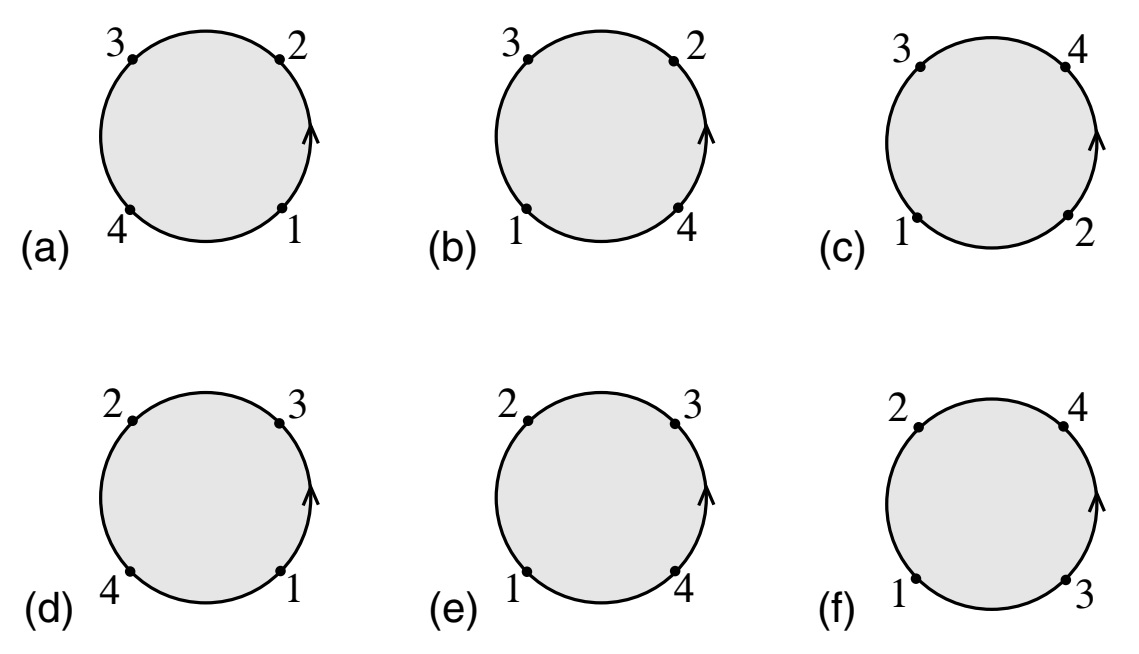
\includegraphics[width=0.5\textwidth,natwidth=854.25,natheight=490.5]{Fig6.2.jpg}\\
		\caption{圆上4个开弦顶点算符的6个循环不等价编序. 除了在点3从$\infty$跃变到$-\infty$, 坐标$y$沿着箭头方向增长.}\label{fig:6.2}
	\end{center}
\end{figure}
	

积分分裂成三部分, $-\infty<y_{4}<0$, $0<y_{4}<1$, 以及 $1<y_{4}<\infty $.  对于这三个范围, 顶点算符的排序如图\ref{fig:6.2}(a)(b)(c)所示. 
M\"{o}bius 不变性可用于将这些范围变至其他任意一个, 所以它们给出的贡献等效于顶点算符的置换.  $(t \leftrightarrow s)$ 项给出图\ref{fig:6.2}(d)(e)(f). 
合起来
\begin{equation}
	S_{D_{2}}(k_{1} ; k_{2} ; k_{3} ; k_{4})=2 \mi g_{\mathrm{o}}^{4} C_{D_{2}}(2 \pi)^{26} \delta^{26}({\textstyle\sum_{i} k_{i}})
	[I(s, t)+I(t, u)+I(u, s)] \:, \label{6.4.9}
\end{equation}
其中
\begin{equation}
	I(s, t)=\int_{0}^{1} \dif y\: y^{-\alpha^{\prime} s-2}(1-y)^{-\alpha^{\prime} t-2}  \:. \label{6.4.10}
\end{equation}
这三项分别来自于图\ref{fig:6.2}的(c)(f)、(b)(d)和(a)(e).

如果$\alpha^{\prime} s<-1$ 并且 $\alpha^{\prime} t<-1$, 积分 $I(s,t)$ 收敛. 当 $\alpha^{\prime} s \rightarrow-1$, 积分在$y=0$发散. 
为研究这一发散, 取 $y=0$ 邻域并对被积函数做近似:
	\begin{align}
		I(s, t) &=\int_{0}^{r} d y y^{-\alpha^{\prime} s-2}+\text{在$\alpha^{\prime} s=-1$处解析的项}   \nonumber \\
		&=-\frac{r^{-\alpha^{\prime} s-1}}{\alpha^{\prime} s+1}+\text{在$\alpha^{\prime} s=-1$处解析的项} \nonumber\\
		&=-\frac{1}{\alpha^{\prime} s+1}+\text{在$\alpha^{\prime} s=-1$处解析的项} \:. \label{6.4.11}
	\end{align}
在\eqref{6.4.11}中, 我们已经计算收敛区域的积分. 我们看到这一发散是$s=-1 / \alpha^{\prime}$处的极点, 开弦快子的质量平方. 
变量$s$正是散射 $1+2 \rightarrow 3+4$的质心能量平方, 所以这一极点是中间快子态所产生的共振. 再一次, 这是玻色弦的人工制品, 即最轻弦态是快子态, 与讨论无关. 
这一极点是由于图\ref{fig:6.3}(a)中的过程. 其中, 快子1和2合并变成单个快子, 然后又分离成快子3和4.

\begin{figure}[h]
	\begin{center}
		%width=0.8\textwidth,bb=0 0 1193 329
		%1px=0.75pt
		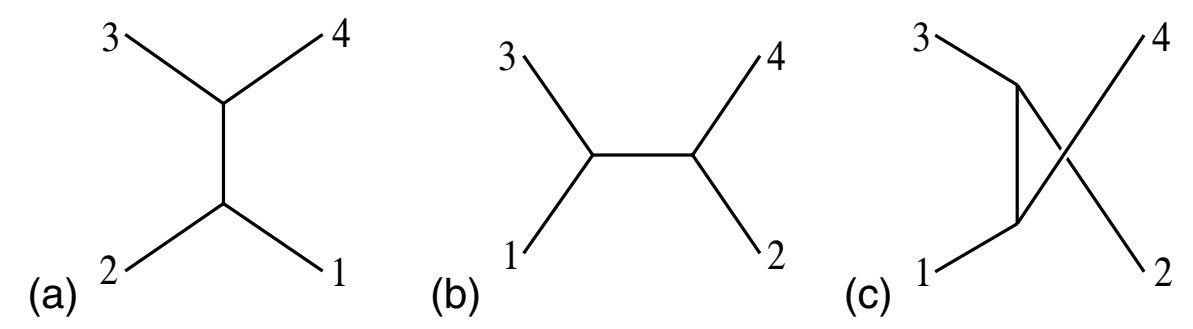
\includegraphics[width=0.5\textwidth,natwidth=894.75,natheight=246.75]{Fig6.3.jpg}\\
		\caption{在(a) $s$-, (b) $t$-, 和(c) $u$-道给出极点的过程.}\label{fig:6.3}
	\end{center}
\end{figure}

由于 $\alpha^{\prime} s=-1$ 处的奇异性只是一个极点,  可以对$I(s,t)$做解析延拓绕过这一点, 并深入到 $\alpha^{\prime} s>-1 $的区域. 
这一振幅经由解析延拓定义. 振幅在这个极点处发散是该振幅的一个显著物理特征: 中间弦态沿着长时空距离传播所对应的共振. 
绕过这一极点的发散则不是; 它仅是该振幅这一特定积分表示的人工产物. 延拓不造成任何问题. 事实上, 我们将看到每一弦发散都是这一基本形式, 
所以这种解析延拓移去了所有发散——当然, 要除去极点本身的发散. 极点在实轴上, 我们需要更精准的定义它. 对于闵可夫斯基过程, 正确的 $\epsilon$ 处理是
\begin{equation}
		\frac{1}{\alpha^{\prime} s+1}  \equiv \frac{1}{\alpha^{\prime} s+1+i \epsilon} 
		 \equiv \mathrm{P} \frac{1}{\alpha^{\prime} s+1}- \mi \pi \delta (\alpha^{\prime} s+1) \:, \label{6.4.12}
\end{equation}
其中$\mathrm{P}$ 代表主值. 幺正性(我们会在第\ref{cha:9}章系统地发展它)要求出现这一极点, 并以两个快子到一个弦的散射振幅决定了系数:
\begin{equation}
		S_{D_{2}}(k_{1} ; k_{2} ; k_{3} ; k_{4})= \mi \int \frac{\dif^{26} k}{(2 \pi)^{26}} 
		\frac{S_{D_{2}}(k_{1} ; k_{2} ; k) S_{D_{2}}(-k ; k_{3} ; k_{4})}{-k^{2}+\alpha^{\prime-1}+ \mi \epsilon} 
		+\text{ 在$k^{2}=\frac{1}{\alpha^{\prime}}$处解析的项}\:. \label{6.4.13}
\end{equation}

将4快子振幅中的因素汇聚一起, 包括$I(u, s)$对这一极点的等价贡献, 并使用3快子结果\eqref{6.4.4}, 条件\eqref{6.4.13}给出
\begin{equation}
	C_{D_{2}}=\me^{-\lambda} C_{D_{2}}^{X} C_{D_{2}}^{\mathrm{g}}=\frac{1}{\alpha^{\prime} g_{\mathrm{o}}^{2}} \:. \label{6.4.14}
\end{equation}
\begin{tcolorbox}
	\begin{remark}
		\eqref{6.4.13}给出的奇异项: 
		\[
		\mi \cdot(2 \mi g_{\mathrm{o}}^{3} C_{D_{2}})^{2}(2 \pi)^{26} \alpha^{\prime} 
		\delta^{2 b}({\textstyle\sum_{i} k_{i}}) \frac{1}{\alpha^{\prime} s+1} \:,
		\]
		\eqref{6.4.9}给出的奇异项: 
		\[
		2 \cdot 2 \mi g_{\mathrm{o}}^{4} C_{D_{2}}(2 \pi)^{26} \delta^{26}({\textstyle\sum_{i} k_{i}}) \frac{-1}{\alpha^{\prime} s+1}\:.
		\]
		二者联立给出\eqref{6.4.14}.
		\end{remark}
\end{tcolorbox}
\noindent 那么3快子振幅是
\begin{equation}
	S_{D_{2}}(k_{1} ; k_{2} ; k_{3})=\frac{2 \mi g_{\mathrm{o}}}{\alpha^{\prime}}(2 \pi)^{26} \delta^{26}({\textstyle\sum_{i} k_{i}}) \:. 
	\label{6.4.15}
\end{equation}
各种泛函行列式被扔掉了. 利用幺正性, 所有归一化可以用出现在顶点算符中的耦合 $g_{o}$ 表示. 
实际上, 行列式也可通过仔细的正规化与重整化算出, 并且不同拓扑的相对归一化与通过幺正性得出的结果一致.

解析延拓绕过极点, 我们遇到了进一步的奇异性. 在 $y=0$ 处展开被积函数
\begin{equation}
	I(s, t)=\int_{0}^{r} \dif y\: \Bigl[y^{-\alpha^{\prime} s-2}+ (\alpha^{\prime} t+2) y^{-\alpha^{\prime} s-1}+\cdots\Bigr] \:. 
	\label{6.4.16}
\end{equation}
第二项给出了$\alpha^{\prime} s=0$处的极点
\begin{equation}
	I(s, t)=\frac{u-t}{2 s}+\text{在$\alpha^{\prime} s=0$处解析的项} \:. \label{6.4.17}
\end{equation}
从泰勒展开后面的项中, 振幅的极点在
\begin{equation}
	\alpha^{\prime} s=-1,0,1,2, \ldots \:. \label{6.4.18}
\end{equation}
它们精确是开弦态的位置. 积分 $I(s, t)$ 关于变量 $t$在相同位置\eqref{6.4.18}有极点, 它们来自于端点 $y=1$.  
这是由于图\ref{fig:6.3}(b)的过程. 振幅\eqref{6.4.9}中的其他两项给出了 $s$道和 $t$ 道和$u$ 道极点(图\ref{fig:6.3}c). 
因为\eqref{6.4.17}在 $s=0$留数对 $u-t$是奇的, 这一极点实际上会与 $I(s, u)$中的极点抵消.  
$1 / \alpha^{\prime}$偶数倍处的奇点都有这样的行为. 但对于下一节要引入的更一般的开弦理论, 这不再成立.

定义欧拉 beta 函数
\begin{equation}
	B(a, b)=\int_{0}^{1} \dif y\: y^{a-1}(1-y)^{b-1} \:, \label{6.4.19}
\end{equation}
使得
\begin{equation}
	I(s, t)=B(-\alpha_{\mathrm{o}}(s),-\alpha_{\mathrm{o}}(t)), \qquad \alpha_{\mathrm{o}}(x)=1+\alpha^{\prime} x \:. 
	\label{6.4.20}
\end{equation}
这可以表达为gamma函数. 对于固定的$w$, 定义 $y=v / w$, 这给出 
\begin{equation}
	w^{a+b-1} B(a, b)=\int_{0}^{w} \dif v \: v^{a-1}(w-v)^{b-1} \:. \label{6.4.21}
\end{equation}
两边乘以$\me^{-w}$并积分 $\int_{0}^{\infty} \dif w$, 重新组合给出
\begin{align}
	\Gamma(a+b) B(a, b) &=\int_{0}^{\infty} \dif v\: v^{a-1} \me^{-v} \int_{0}^{\infty} \dif(w-v) \: (w-v)^{b-1} \me^{-(w-v)} \nonumber \\
	&=\Gamma(a) \Gamma(b) \:. \label{6.4.22}
\end{align}
那么4快子振幅就是
\begin{align}
	&S_{D_{2}}(k_{1}; k_{2} ; k_{3} ; k_{4})=\frac{2 \mi g_{\mathrm{o}}^{2}}{\alpha^{\prime}}
	(2 \pi)^{26} \delta^{26}({\textstyle \sum_{i} k_{i}}) \nonumber \\
	&\qquad \times\Bigl[B(-\alpha_{\mathrm{o}}(s),-\alpha_{\mathrm{o}}(t))+B(-\alpha_{\mathrm{o}}(s),-\alpha_{\mathrm{o}}(u))
	+B(-\alpha_{\mathrm{o}}(t),-\alpha_{\mathrm{o}}(u))\Bigr] \:, \label{6.4.23}
\end{align}
其中
\begin{equation}
	B(-\alpha_{\mathrm{o}}(x),-\alpha_{\mathrm{o}}(y))=
	\frac{\Gamma(-\alpha^{\prime} x-1) \Gamma(-\alpha^{\prime} y-1)}{\Gamma(-\alpha^{\prime} x-\alpha^{\prime} y-2)} \:. \label{6.4.24}
\end{equation}
这是Veneziano振幅, 最早是为了模拟强相互作用的某些特征而写下的.

Veneziano振幅的高能行为是重要的. 有两个感兴趣的区域, Regge极限,
\begin{equation}
	s \rightarrow \infty, \quad t \text{ 固定} \:, \label{6.4.25}
\end{equation}
以及硬散射极限
\begin{equation}
	s \rightarrow \infty, \quad t / s \text{ 固定} \:. \label{6.4.26}
\end{equation}
如果我们考虑散射过程$1+2 \rightarrow 3+4$ (使得 $k_{1}^{0}$ 和$k_{2}^{0}$ 是正的, 而 $k_{3}^{0}$ 和 $k_{4}^{0}$ 是负的), 
那么在 $1$-$2$ 质心系中,
\begin{equation}
	s=E^{2}, \quad t=(4 m^{2}-E^{2}) \sin^{2}\frac{\theta}{2}, \quad u=(4 m^{2}-E^{2}) \cos ^{2} \frac{\theta}{2} \:, \label{6.4.27}
\end{equation}
其中 $E$ 是质心系能量, 而$\theta$ 是粒子1与3之间夹角. Regge极限是高能与小角度, 而硬散射极限是高能与固定角. 利用Stirling近似, 
$\Gamma(x+1) \approx x^{x} \me^{-x}(2 \pi x)^{1 / 2}$, Regge 区域的行为是
\begin{equation}
	S_{D_{2}}(k_{1} ; k_{2} ; k_{3} ; k_{4}) \propto s^{\alpha_{\mathrm{o}}(t)} \Gamma(-\alpha_{0}(t)) \:, \label{6.4.28}
\end{equation}
其中$\alpha_{\mathrm{o}}(t)=\alpha^{\prime} t+1 $, 即振幅按照$s$的幂次变化, 而幂次依赖于$t$. 这是Regge行为. 
在gamma函数的极点振幅是$s$的整数次幂, 对应于交换整数自旋 $\alpha_{o}(t)$的弦.

在硬散射极限下
\begin{equation}
	S_{D_{2}}(k_{1} ; k_{2} ; k_{3} ; k_{4}) \approx \exp \bigl[-\alpha^{\prime}(s \ln s \alpha^{\prime}+t \ln t \alpha^{\prime}+u \ln u \alpha^{\prime})\bigr]=\exp [-\alpha^{\prime} s f(\theta)] \:, \label{6.4.29}
\end{equation}
其中
\begin{equation}
	f(\theta) \approx-\sin ^{2} \frac{\theta}{2} \ln \sin ^{2} \frac{\theta}{2}-\cos ^{2} \frac{\theta}{2} \ln \cos ^{2} \frac{\theta}{2}
	\label{6.4.30}
\end{equation}
是正的.  \eqref{6.4.29}值得注意. 高能、固定角散射探查了被散射物体的内部结构. Rutherford用硬$\alpha$原子散射发现了原子核.  
SLAC上的电子-核子硬散射揭示了核子的夸克组分. 在量子场论中, 硬散射振幅按$s $幂次衰减. 即使是像核子这样的复合物体, 如果它的组分是类点的, 它也是幂次律振幅 . 
指数衰减\eqref{6.4.29}则软的多, 体现了一个尺寸为$\alpha^{1 / 2}$的物体, 这是我们所期待的. 

我们从三点振幅开始, 跳过了零点、一点和两点振幅. 我们会在\ref{sec:6.6}节讨论这些振幅以及它们的解释 .

\section{Chan-Paton因子和规范相互作用} \label{sec:6.5}%{6.5 Chan-Paton factors and gauge interactions}

在本节我们将考察开弦无质量矢量态的相互作用. 为了使这个讨论有趣些, 我们首先来推广开弦理论.

在第\ref{cha:3}章末尾, 我们引入了一大类玻色弦理论, 但对相互作用的初步考察中, 我们集中于26维平坦时空的简单情况. 
可以用对称性的方式思考它: 这一理论有极大的26维庞加莱不变性. 在玻色闭弦中, 这是拥有这一对称性的唯一理论. 
证明的概述如下: 时空平移的世界面诺特流有权重为(1,0)和(0,1)的分量.  通过\ref{sec:2.9}节所给出的讨论, 
这些流关于$z$或$\bar{z}$是全纯的. 在本章的计算中, 这足以决定所有期望值.

然而, 在开弦理论中存在一个推广. 开弦有边界, 端点. 在含有可区分端点的量子系统中, 除了在块中传播的场外, 在这些点上很自然地含有自由度. 
在开弦的每一端点, 我们增加新的自由度, 称为Chan-Paton自由度, 它可以是 $n$ 个态中的一个. 那么弦态的基是
\begin{equation}
	|N ; k ; i j\rangle \:, \label{6.5.1}
\end{equation}
其中 $i$ 和 $j$ 标记左端点和右端点的态, 从1取到$n$. 能动量张量像往常那样定义, 对新自由度没有依赖关系. 因而, 共形不变性是自动的. 
正如Chan-Paton自由度是不变的, 庞加莱不变性也是自动的. 尽管这些新自由度的世界面动力学很平庸, 但对于时空物理, 它们有深远的影响. 

\begin{figure}[h]
	\begin{center}
		%width=0.8\textwidth,bb=0 0 529 156
		%1px=0.75pt
		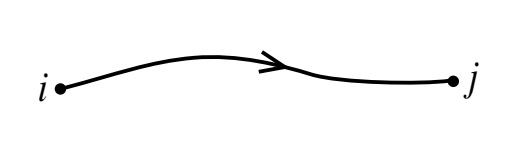
\includegraphics[width=0.5\textwidth,natwidth=396.75,natheight=117]{Fig6.4.jpg}\\
		\caption{带有Chan--Paton自由度的开弦}\label{fig:6.4}
	\end{center}
\end{figure}

在强相互作用的弦理论中, 引入Chan-Paton因子的动机是为了引入$S U(3)$ 味量子数: 端点就像夸克和反夸克, 通过色-电流管相连接. 现在我们在更广泛的框架下引入它: 考察所有可能的对称性. 在第\ref{cha:8}章, 我们将给Chan-Paton自由度一个新解释, 在第14章将附加一个可能的进一步的改进 .

现在有 $n^{2}$ 个标量快子, $n^{2}$ 个无质量矢量玻色子, 以此类推. 引入$n^{2}$个厄米矩阵$\lambda_{i j}^{a}$, 并做归一化
\begin{equation}
	\operatorname{Tr}(\lambda^{a} \lambda^{b})=\delta^{a b} \:, \label{6.5.2}
\end{equation}
这些矩阵是两个端点的态的完备基. 它们是$U(n)$的表示矩阵, 所以可以猜测无质量矢量玻色子与 $U(n)$ 对称性相联系; 一会儿我们就会看到确实是这种情况.

定义基
\begin{equation}
	|N ; k ; a\rangle=\sum_{i, j=1}^{n}|N ; k ; i j\rangle \lambda_{i j}^{a}  \:. \label{6.5.3}
\end{equation}
现在考察图 \ref{fig:6.2}(a)所示的4快子振幅, 在这个图中, 顶点算符按循环序1234排列. 因为Chan-Paton自由度没有出现在哈密顿量, 
它们的态在顶点算符之间无法演化: 快子1右端点的态必须与快子2左端点的态相同, 剩余的情况以此类推. 因此, 振幅 \ref{fig:6.2}(a) 将会包含因子
\begin{equation}
	\operatorname{Tr}(\lambda^{a_{1}} \lambda^{a_{2}} \lambda^{a_{3}} \lambda^{a_{4}}) \:, \label{6.5.4}
\end{equation}
这个因子来自于每个快子的Chan-Paton波函数的重叠. 这一规则可以推广至任意振幅: 每一顶点算符现在包含来自端点自由度波函数的 Chan-Paton 因子 $\lambda_{i j}^{a}$, 
而每一世界面的振幅要乘以沿着边界的Chan-Paton因子的迹.

3快子振幅变成
\begin{align}
	S_{D_{2}}(k_{1}, a_{1} ; k_{2}, a_{2} ; k_{3}, a_{3})= 
	 \frac{\mi g_{\mathrm{o}}}{\alpha^{\prime}}(2 \pi)^{26} \delta^{26}({\textstyle\sum_{i} k_{i}}) 
	 \operatorname{Tr}(\lambda^{a_{1}} \lambda^{a_{2}} \lambda^{a_{3}}+\lambda^{a_{1}} \lambda^{a_{3}} \lambda^{a_{2}}) \:, \label{6.5.5}
\end{align}
两个轮换序现在有了不同的Chan-Paton迹. 4快子振幅是
	\begin{align}
		&S_{D_{2}}(k_{1}, a_{1} ; k_{2}, a_{2} ; k_{3}, a_{3} ; k_{4}, a_{4})
		=\frac{\mi g_{\mathrm{o}}^{2}}{\alpha^{\prime}}(2 \pi)^{26} \delta^{26}({\textstyle \sum_{i} k_{i}}) \nonumber \\
		&\quad \times \Bigl[\operatorname{Tr}(\lambda^{a_{1}} \lambda^{a_{2}} \lambda^{a_{4}} \lambda^{a_{3}}
		+\lambda^{a_{1}} \lambda^{a_{3}} \lambda^{a_{4}} \lambda^{a_{2}}) B(-\alpha_{\mathrm{o}}(s),-\alpha_{\mathrm{o}}(t)) \nonumber  \\
		&\qquad+\operatorname{Tr}(\lambda^{a_{1}} \lambda^{a_{3}} \lambda^{a_{2}} \lambda^{a_{4}}
		+\lambda^{a_{1}} \lambda^{a_{4}} \lambda^{a_{2}} \lambda^{a_{3}}) B(-\alpha_{\mathrm{o}}(t),-\alpha_{\mathrm{o}}(u))\nonumber \\
		&\qquad+\operatorname{Tr}(\lambda^{a_{1}} \lambda^{a_{2}} \lambda^{a_{3}} \lambda^{a_{4}}
		+\lambda^{a_{1}} \lambda^{a_{4}} \lambda^{a_{3}} \lambda^{a_{2}}) 
		B(-\alpha_{\mathrm{o}}(s),-\alpha_{\mathrm{o}}(u))\Bigr] \:. \label{6.5.6}
	\end{align}
再次考察幺正性关系\eqref{6.4.13}, 在$s=-1 / \alpha^{\prime}$ 处的极点使得左边获得因子
\begin{equation}
	\frac{1}{4} \operatorname{Tr}\Bigl(\{\lambda^{a_{1}}, \lambda^{a_{2}}\} \{\lambda^{a_{3}}, \lambda^{a_{4}}\}\Bigr) \:,\label{6.5.7}
\end{equation}
而右边获得因子
\begin{equation}
	\frac{1}{4} \sum_{a} \operatorname{Tr}\Bigl(\{\lambda^{a_{1}}, \lambda^{a_{2}}\} \lambda^{a}\Bigr) 
	\operatorname{Tr}\Bigl(\{\lambda^{a_{3}}, \lambda^{a_{4}}\} \lambda^{a}\Bigr) \:, \label{6.5.8}
\end{equation}
即对中间态的Chan-Paton波函数求和.  $\lambda_{i j}^{a}$ 的完备性与归一化\eqref{6.5.2}暗示了对于任意的$A$和$B$, 有
\begin{equation}
	\operatorname{Tr}(A \lambda^{a}) \operatorname{Tr}(B \lambda^{a})=\operatorname{Tr}(A B) \:,  \label{6.5.9}
\end{equation}
因而振幅依旧是幺正的.

\begin{tcolorbox}
	\begin{proof}
		记$\operatorname{Tr}(A \lambda^{a})=\langle A \vert \lambda^{a}\rangle=\langle\lambda^{a}|A\rangle$, 那么
		\[
		\operatorname{Tr}(A \lambda^{a}) \operatorname{Tr}(B \lambda^{a}) = 
		\langle A \vert \lambda^{a}\rangle\langle\lambda^{\alpha} \vert B\rangle=\langle A \vert B\rangle \:,
		\]
		其中 $\sum_{a}|\lambda^{a}\rangle\langle\lambda^{a}|=1$ 来自于 $\langle\lambda^{a} \vert \lambda^{b}\rangle= \delta^{a b}$.
	\end{proof}	
\end{tcolorbox}



\subsection*{规范相互作用}
一个规范玻色子与两个快子的振幅是	
\begin{align}
	&S_{D_{2}}(k_{1}, a_{1}, e_{1} ; k_{2}, a_{2} ; k_{3}, a_{3})= 
	-\mi g_{\mathrm{o}}^{\prime} g_{\mathrm{o}}^{2} \me^{-\lambda} e_{1 \mu} \nonumber \\
	&\quad \times\Bigl\langle \bno c^{1} \dot{X}^{\mu} \me^{\mi k_{1} \cdot X}(y_{1})\bno 
	 \bno  c^{1} \me^{\mi k_{2} \cdot X}(y_{2})\bno \bno c^{1} \me^{\mi k_{3} \cdot X}(y_{3})\bno\Bigr\rangle_{D_{2}} 
	\operatorname{Tr}(\lambda^{a_{1}} \lambda^{a_{2}} \lambda^{a_{3}})  \nonumber\\
	&\qquad \qquad +(k_{2}, a_{2}) \leftrightarrow(k_{3}, a_{3}) \:. \label{6.5.10}
\end{align}
我们使用了玻色顶点算符\eqref{3.6.26}, 但暂且允许一个独立的归一化常数 $g_{\mathrm{o}}^{\prime}$. 利用\ref{sec:6.2}节结果,  
$X$的路径积分是
\begin{align}
	&\Bigl\langle \bno \dot{X}^{\mu} \me^{\mi k_{1} \cdot X}(y_{1})\bno \bno \me^{\mi k_{2} \cdot X}(y_{2})\bno 
	\bno \me^{\mi k_{3} \cdot X}(y_{3})\bno \Bigr\rangle_{D_{2}} 
	=-2 \mi \alpha^{\prime}\biggl(\frac{k_{2}^{\mu}}{y_{12}}+\frac{k_{3}^{\mu}}{y_{13}}\biggr) \nonumber \\
	&\qquad \times \mi C_{D_{2}}^{X}(2 \pi)^{26} \delta^{26}({\textstyle \sum_{i} k_{i}})
	|y_{12}|^{2 \alpha^{\prime} k_{1} \cdot k_{2}}|y_{13}|^{2 \alpha^{\prime} k_{1} \cdot k_{3}} 
	|y_{23}|^{2 \alpha^{\prime} k_{2} \cdot k_{3}} \:. \label{6.5.11}
\end{align}
利用动量守恒、质壳条件, 以及物理态条件$k_{1} \cdot e_{1}=0$, 振幅变成
\begin{align}
	&S_{D_{2}}(k_{1}, a_{1}, e_{1} ; k_{2}, a_{2} ; k_{3}, a_{3}) \nonumber \\
	&=-\mi g_{\mathrm{o}}^{\prime} e_{1} \cdot k_{23}(2 \pi)^{26} \delta^{26}({\textstyle \sum_{i} k_{i}}) 
	\operatorname{Tr}\Bigl(\lambda^{a_{1}}[\lambda^{a_{2}}, \lambda^{a_{3}}]\Bigr) \:, \label{6.5.12}
\end{align}
其中 $k_{i j} \equiv k_{i}-k_{j} $.  这又一次独立于顶点算符的位置.

4快子振幅中的 $s=0$ 极点不再为零. 被抵消的那一项现在有次序不同的Chan-Paton因子, 因此极点正比于
\begin{equation}
	\operatorname{Tr}\Bigl([\lambda^{a_{1}}, \lambda^{a_{2}}][\lambda^{a_{3}}, \lambda^{a_{4}}]\Bigr) \:. \label{6.5.13}
\end{equation}
通过幺正性将这一极点的系数与振幅\eqref{6.5.12}相关联, 获得
\begin{equation}
	g_{\mathrm{o}}^{\prime}=(2 \alpha^{\prime})^{-1 / 2} g_{\mathrm{o}} \:. \label{6.5.14}
\end{equation}
这与从态算符映射导出的相对归一化相同: 仅存在一个独立的耦合常数. 

对于3规范玻色子耦合, 一个类似的计算给出
\begin{align}
	&S_{D_{2}}(k_{1}, a_{1}, e_{1} ; k_{2}, a_{2}, e_{2} ; k_{3}, a_{3}, e_{3}) \nonumber \\
	&\qquad = \mi g_{\mathrm{o}}^{\prime}(2 \pi)^{26} \delta^{26}({\textstyle\sum_{i} k_{i}})
	\Bigl(e_{1} \cdot k_{23} e_{2} \cdot e_{3}+e_{2} \cdot k_{31} e_{3} \cdot e_{1}+e_{3} \cdot k_{12} e_{1} \cdot e_{2} \nonumber\\
	&\qquad \qquad +\frac{\alpha^{\prime}}{2} e_{1} \cdot k_{23} e_{2} \cdot k_{31} e_{3} \cdot k_{12} \Bigr) 
	\operatorname{Tr}\Bigl(\lambda^{a_{1}}[\lambda^{a_{2}}, \lambda^{a_{3}}]\Bigr) \:. \label{6.5.15}
\end{align}

至动量的一阶, 我们所发现的振幅可以通过如下时空作用量重新产生: 
\begin{equation}
		\bm{S}=\frac{1}{g_{\mathrm{o}}^{\prime 2}} \int \dif^{26} x\: \biggl[-\frac{1}{2} \operatorname{Tr}(D_{\mu} \varphi D^{\mu}\varphi)+\frac{1}{2 \alpha^{\prime}} \operatorname{Tr}(\varphi^{2})+\frac{2^{1 / 2}}{3 \alpha^{\prime 1 / 2}} 
		\operatorname{Tr}(\varphi^{3})
		-\frac{1}{4} \operatorname{Tr}(F_{\mu \nu} F^{\mu \nu})\biggr] \:, \label{6.5.16}
\end{equation}
其中快子场 $\varphi$ 与杨-米尔斯矢势 $A_{\mu}$ 被写成了 $n \times n$ 矩阵, 即 $A_{\mu}=A_{\mu}^{a} \lambda^{a} $. 
另外, $D_{\mu} \varphi=\partial_{\mu} \varphi-\mi[A_{\mu}, \varphi]$, 
并且 $F_{\mu \nu}=\partial_{\mu} A_{\nu}-\partial_{\nu} A_{\mu}-\mi[A_{\mu}, A_{\nu}]$.

这是$U(n)$规范场在伴随表示下与标量场相耦合的作用量. Chan-Paton因子中所增加的恰好就是规范不变表示需要的. 由于在弦微扰论中会保证非物理态的退耦, 规范不变性是自动的, 我们将会进一步研究它.

在远小于弦尺度的动量$k$处, 唯一的开弦态是无质量规范玻色子. 正如\ref{sec:3.7}节讨论的, 在这一极限下, 物理应该约化至无质量态的有效场论. 
因此, 在作用量\eqref{6.5.16}中引入快子必有某些地方不合逻辑; 我们这样做是为了启发. 但现在让我们专注于规范玻色子. 
4规范玻色子的振幅形式类似于 Veneziano 振幅, 但含有来自极化张量的额外结构. 将其展成$\alpha^{\prime} k^{2}$的幂级数, 第一项会在零斜率极限下幸存, 
它是$s, t, u$处的极点项和加上一个常数. 相容性会保证它与通过场论中的杨-米尔斯拉格朗日量$F_{\mu \nu} F^{\mu\nu} $所获得的4规范玻色子振幅精确相同. 
然而, 注意到3规范玻色子振幅\eqref{6.5.15}的$\alpha^{\prime} k^{3}$ 阶项. 这暗示了拉格朗日量中的高阶导数项
\begin{equation}
	-\frac{2 \mi \alpha^{\prime}}{3 g_{\text{o}}^{\prime 2}} \operatorname{Tr}(F_{\mu}{}^{\nu} F_{\nu}{}^{\omega} F_{\omega}{}^{\mu}) \:.
	\label{6.5.17}
\end{equation}
类似地, 展开4点振幅会揭示出高阶相互作用的无限和(除了\eqref{6.5.17}, 它们确实对3规范玻色子振幅没有运动学方面贡献). 
在低能区域, 弦的圈振幅也会约化至从有效拉格朗日量中获得的圈.  经由有效拉格朗日量的通用逻辑, 高阶导数项在低能处不是很重要, 
它们在标度 $\alpha^{\prime} k^{2} \approx 1$变得重要, 这个标度正是新物理(有质量弦态)出现的地方, 而有效作用量不再适用.

如果我们有一个截断, 为什么还需要重整化? 重整化依旧拥有内涵. 并且事实上这是它真实的解释: 它意味着, 除了有效拉格朗日量中的参量外, 低能物理与高能物理的细节无关. 
这是喜忧参半的: 它意味着我们可以在不知道普朗克标度处的理论的情况下, 利用普通的量子场论在加速器的能量级别做出预测, 
但它也意味着我们无法用粒子加速器处的物理探测普朗克能标处的理论.

弦频谱与振幅有一个显然的整体$U(n)$对称性,
\begin{equation}
	\lambda^{a} \rightarrow U \lambda^{a} U^{\dagger} \:, \label{6.5.18}
\end{equation}
它保持 Chan-Paton迹以及态的范数不变. 从振幅的细节, 我们看到这实际上时空的定域对称性. 我们将看到从整体世界面对称性到定域时空对称性的提升在弦论中是十分普遍的现象.

所有开弦态按照$U(n)$对称性下的 $n \times n$ 伴随表示变换. 顺带地, $U(n)$ 不是单李代数: $U(n)=S U(n) \times U(1) $. 
$U(1)$的规范玻色子, $\lambda_{i j}=\delta_{i j} / n^{1 / 2}$, 从振幅\eqref{6.5.12}和\eqref{6.5.15}中退耦. 
$U(1)$的伴随表示是平庸的, 所以所有弦态在$U(1)$对称下是中性的.

\subsection*{非定向弦}

推广到非定向弦是有趣的. 首先考虑没有Chan-Paton因子的理论. 除了 M\"{o}bius 不变性外, 球面或圆盘上的$X^{\mu}$CFT 在开弦的方向反射对称性 $\sigma^{1} \rightarrow \pi-\sigma^{1}$或是闭弦上的$\sigma^{1} \rightarrow 2 \pi-\sigma^{1}$下是不变的. 
世界面宇称由算符 $\Omega$ 生成. 从模式展开得出, 在开弦中
\begin{equation}
	\Omega \alpha_{n}^{\mu} \Omega^{-1}=(-1)^{n} \alpha_{n}^{\mu} \:, \label{6.5.19}
\end{equation}
在闭弦中
\begin{equation}
	\Omega \alpha_{n}^{\mu} \Omega^{-1}=\tilde{\alpha}_{n}^{\mu} \:. \label{6.5.20}
\end{equation}
这一对称性同时扩展到鬼场.但为了集中注意力, 我们这里不讨论它们, 它们对树图的贡献也仅仅是个固定的因子. 

无论开弦还是闭弦, 快子顶点算符在世界面宇称下是偶的 (这对于无鬼的被积顶点算符是显然的; 那么固定的算符也必须以同样的方式变换), 这决定了算符的符号. 
那么所有的态可以根据它们的宇称本征值 $\omega=\pm 1 $分类.  开弦中的关系\eqref{6.5.19}暗示了
\begin{equation}
	\Omega|N ; k\rangle=\omega_{N}|N ; k\rangle, \quad \omega_{N}=(-1)^{1+\alpha^{\prime} m^{2}} \:. \label{6.5.21}
\end{equation}
世界面宇称是乘积守恒. 例如, 3快子振幅非零, 与 $(+1)^{3}=1$ 相容.  另一方面, 无质量矢量有 $\omega=-1$, 所以我们可以预期在没有Chan-Paton因子时, 
矢量-快子-快子振幅\eqref{6.5.10}与3矢量振幅\eqref{6.5.15}为零, 结果也确实如此 ($\lambda^{a}$ 被替换成1, 而对易子为零). 
不同的轮换顺序, 也通过世界面宇称彼此相关, 因而相互抵消.

给定一个相容的定向弦论, 通过将频谱限制在$\omega=+1$的态上, 我们给出了新的非定向弦论.  $\alpha^{\prime} m^{2}$ 为奇的态保留, 
而 $\alpha^{\prime} m^{2}$为偶的态, 包括光子, 被禁止了. $\omega$ 守恒保证了, 如果所有的外态有$\omega=+1$, 那么树图的中间态也有 $\omega=+1$. 
因此, 至少在树图级, 非定向弦的幺正性从定向弦的幺正性得出. 

对于非定向理论的主要兴趣就在于Chan-Paton因子的处理. 由于我们能识别出开弦的相对端点, 世界面宇称必会反转它们
\begin{equation}
	\Omega|N ; k ; i j\rangle=\omega_{N}|N ; k ; j i\rangle \:. \label{6.5.22}
\end{equation}
再一次, 这是定向理论中所有振幅的一个对称性. 为了构成非定向理论, 我们再一次将频谱约束到世界面宇称本征值 $\omega=+1 $. 
取 $\lambda_{i j}^{a}$ 的一组基, 使得每个矩阵要么对称 $s^{a}=+1$;要么反对称,  $s^{a}=-1$. 那么
\begin{equation}
	\Omega|N ; k ; a\rangle=\omega_{N} s^{a}|N ; k ; a\rangle \:. \label{6.5.23}
\end{equation}
世界面宇称本征值是 $\omega=\omega_{N} s^{a}$, 那么非定向频谱是
\begin{subequations} \label{6.5.24}
\begin{align}
&\text{偶数倍的}\alpha^{\prime} m^{2} \:: \qquad   \text{反对称的 } \lambda^{a}  \:, \label{6.5.24a} \\ 	
&\text{奇数倍的}\alpha^{\prime} m^{2} \:: \qquad   \text{\phantom{反}对称的 } \lambda^{a}  \:. \label{6.5.24b} 
\end{align}			
\end{subequations}
对于无质量规范玻色子, Chan-Paton因子是 $n \times n$ 反对称矩阵, 所以规范群是 $S O(n) $.  偶数质量能级的态按照正交群 $S O(n)$的伴随表示变换, 而奇数质量能级的态按照无迹对称张量加一个单态表示变换.

定向理论有一大类方向反演对称性, 它们作为 $\Omega$ 与 $U(n)$ 旋转的组合获得
\begin{equation}
	\Omega_{\gamma}|N ; k ; i j\rangle=\omega_{N} \gamma_{j j^{\prime}}\left|N ; k ; j^{\prime} i^{\prime}\right\rangle \gamma_{i^{\prime} i}^{-1} \:. \label{6.5.25}
\end{equation}
通过将频谱约束至 $\omega_{y}=+1$,我们可以构造更加普遍的非定向理论. 这又一次与相互作用是相容的, 用 $\Omega_{\gamma}$ 作用两次给出
\begin{equation}
	\Omega_{\gamma}^{2}|N ; k ; i j\rangle= [(\gamma^{T})^{-1} \gamma]_{i i^{\prime}}
	|N ; k ; i^{\prime} j^{\prime}\rangle (\gamma^{-1} \gamma^{T})_{j^{\prime} j} \:. \label{6.5.26}
\end{equation}
我们假定 $\Omega_{\gamma}^{2}=1$ , 原因会在下面解释. 这暗示了
\begin{equation}
	\gamma^{T}=\pm \gamma \:. \label{6.5.27}
\end{equation}
即, $\gamma$是对称或反对称的.

Chan-Paton的基变换是
\begin{equation}
	|N ; k ; i j\rangle^{\prime}=U_{i i^{\prime}}^{-1} |N ; k ; i^{\prime} j^{\prime}\rangle U_{j^{\prime} j} \:, \label{6.5.28}
\end{equation}
这将 $\gamma$变到
\begin{equation}
	\gamma^{\prime}=U^{T} \gamma U \:. \label{6.5.29}
\end{equation}
在对称情形下, 总能找到一组基, 使得 $\gamma=1$, 这给出上面已经考察过的情况. 在反对称的情况下, 存在一组基, 使得
\begin{equation}
	\gamma=M \equiv \mi\begin{bmatrix}
		0 & I \\
		-I & 0
	\end{bmatrix} \:. \label{6.5.30}
\end{equation}
这里 $I$ 是 $k \times k$ 单位矩阵, 由于  $\gamma$是可逆反对称矩阵, $n=2 k$ 必须为偶. 我们取Chan-Paton 波函数的一组基, 
使得 $M(\lambda^{a})^{T} M=s^{a^{\prime}} \lambda^{a}$, 其中 $s^{a^{\prime}}=\pm 1$. 
那么世界面本征值是 $\omega_{\gamma}=\omega_{N} s^{a^{\prime}}$, 并且非定向频谱是
\begin{subequations} \label{6.5.31}
\begin{align}
\text{偶数倍的 }\alpha^{\prime} m^{2} \:: \qquad   M(\lambda^{a})^{T} M=-\lambda^{a} \:, \label{6.5.31a} \\
\text{奇数倍的 }\alpha^{\prime} m^{2} \:: \qquad   M(\lambda^{a})^{T} M=+\lambda^{a} \:. \label{6.5.31b}
\end{align}
\end{subequations}
在偶数质量能级, 包括规范玻色子, 这定义了辛群 $S p(k)$ 的伴随表示.

为了构建非定向理论, 我们必须有 $\Omega_{\gamma}^{2}=1$, 理由如下. 既然$\Omega^{2}=1$, 
$\Omega_{\gamma}^{2}$必须仅作用于Chan-Paton因子上. 事实上, 从\eqref{6.5.26}, 它在 Chan-Paton 波函数上的作用为
\begin{equation}
	\lambda \rightarrow (\gamma^{T})^{-1} \gamma \lambda \gamma^{-1} \gamma^{T}=\lambda \:, \label{6.5.32}
\end{equation}
其中, 由于所有的态在$\Omega_{\gamma}$ 下是不变的, 最后一个等号在非定向理论中必须成立. 现在我们断言所允许的 Chan-Paton 波函数必构成完备基. 
关键在于, 两个开弦通过图\ref{fig:3.4}(c)的分裂聚合相互作用可以交换端点. 以这种方式, 可以到达一个完备基, 即到达任一个Chan-Paton 态$|i j\rangle$. 通过 Schur引理, 如果\eqref{6.5.32}对完备基成立, 那么 $\gamma^{-1} \gamma^{T}=1$ , 因而 $\Omega_{\gamma}^{2}=1$.

通过取 $\lambda^{a} $ 的不同集合, 我们可以试图获得不同的规范理论. 事实上, 上面构建的定向 $U(n)$ 理论与非定向的$S O(n)$和 $S p(k)$ 理论是唯一的可能性. 
\eqref{6.5.7} -- \eqref{6.5.9}中完备性讨论的推广表明它们是非定向理论的最一般解. 特别地, 例外李代数无法从Chan-Paton因子获得. 
在闭弦理论中, 有其他机制给出规范玻色子, 并且允许其他群.

\section{闭弦树图振幅} \label{sec:6.6}%{6.6 Closed string tree amplitudes}

关于闭弦振幅的讨论与上面类似. 3闭弦快子的振幅是
\begin{equation}
	S_{S_{2}}(k_{1} ; k_{2} ; k_{3})=g_{\mathrm{c}}^{3} \me^{-2 \lambda}\left\langle\prod_{i=1}^{3} 
	: \mathrel{\tilde{c} c \me^{\mi k_{i} \cdot X}(z_{i}, \bar{z}_{i})}:\right\rangle \bigg._{\!\!S_{2}} \:. \label{6.6.1}
\end{equation}
在这一情况下, CKG $PSL(2, \mathds{C})$ (M\"{o}bius群) 可以将三个顶点算符固定在任意位置 $z_{1,2,3}$. 从\ref{sec:6.2}节中取期望值, 
结果又一次独立于顶点算符,
\begin{equation}
	S_{S_{2}}(k_{1} ; k_{2} ; k_{3})= \mi g_{\mathrm{c}}^{3} C_{S_{2}}(2 \pi)^{26} \delta^{26}({\textstyle \sum_{i} k_{i}}) \:, 
	\label{6.6.2}
\end{equation}
其中 $C_{S_{2}}=\me^{-2 \lambda} C_{S_{2}}^{X} C_{S_{2}}^{\mathrm{g}}$.

对于4闭弦快子
\begin{equation}
	S_{S_{2}}(k_{1} ; k_{2} ; k_{3} ; k_{4})=g_{\mathrm{c}}^{4} \me^{-2 \lambda} 
	\int_{\mathds{C}} \dif^{2} z_{4} \: \left\langle\prod_{i=1}^{3}
	: \mathrel{\tilde{c} c \me^{\mi k_{i} \cdot X}(z_{i}, \bar{z}_{i})}:
	: \mathrel{\me^{\mi k_{4} \cdot X}(z_{4}, \bar{z}_{4})}:\right\rangle\bigg._{\!\!S_{2}} \:, \label{6.6.3}
\end{equation}
其中积分范围为整个复平面$\mathds{C}$. 计算期望值并令 $z_{1}=0, z_{2}=1, z_{3}=\infty$, 这变成
\begin{equation}
	S_{S_{2}}(k_{1} ; k_{2} ; k_{3} ; k_{4}) = 
	\mi g_{\mathrm{c}}^{4} C_{S_{2}}(2 \pi)^{26} \delta^{26}({\textstyle\sum_{i} k_{i}}) J(s, t, u) \:, \label{6.6.4}
\end{equation}
其中
\begin{equation}
	J(s, t, u)=\int_{\mathds{C}} \dif^{2} z_{4}\: |z_{4}|^{-\alpha^{\prime} u / 2-4}|1-z_{4}|^{-\alpha^{\prime} t/2-4}\:. \label{6.6.5}
\end{equation}
这里 $s+t+u=-16 / \alpha^{\prime}$, 我们这里标记出了$J$对所有3个变量的相关性, 这是为了强调它们之间的对称性. 
当$s, t, u<-4 / \alpha^{\prime}$, 振幅收敛. 当 $z_{4} \rightarrow 0$, 它有关于$u$的极点;当 $z_{4} \rightarrow 1$, 它有关于$t$的极点; 
当 $z_{4} \rightarrow \infty$, 它有关于$s$的极点. 这些极点所处位置: 
\begin{equation}
	\alpha^{\prime} s\,,\: \alpha^{\prime} t \,,\: \alpha^{\prime} u=-4,0,4,8, \ldots,\label{6.6.6}
\end{equation}
它们是闭弦态的质量平方. $\alpha^{\prime} s=-4$ 处的极点是
\begin{equation}
	\mi g_{\mathrm{c}}^{4} C_{S_{2}} \int_{|z_{4}|>1 / \epsilon} \dif^{2} z_{4}\: |z_{4}|^{\alpha^{\prime} s / 2} 
	\sim-\frac{8 \pi \mi g_{\mathrm{c}}^{4} C_{S_{2}}}{\alpha^{\prime} s+4} \:. \label{6.6.7}
\end{equation}
幺正性给出
\begin{equation}
	C_{S_{2}}=\frac{8 \pi}{\alpha^{\prime} g_{\mathrm{c}}^{2}} \:, \label{6.6.8}
\end{equation}
因此
\begin{equation}
	S_{S_{2}}(k_{1} ; k_{2} ; k_{3})=\frac{8 \pi \mi g_{\mathrm{c}}}{\alpha^{\prime}}(2 \pi)^{26} 
	\delta^{26}({\textstyle\sum_{i} k_{i}}) \:. \label{6.6.9}
\end{equation}

类似于Veneziano振幅, 4闭弦快子振幅可以表述成gamma 函数:
\begin{equation}
	S_{S_{2}}(k_{1} ; k_{2} ; k_{3} ; k_{4})=\frac{8 \pi \mi g_{\mathrm{c}}^{2}}{\alpha^{\prime}}(2 \pi)^{26} 
	\delta^{26}({\textstyle \sum_{i} k_{i}}) C(-\alpha_{\mathrm{c}}(t),-\alpha_{\mathrm{c}}(u)) \:, \label{6.6.10}
\end{equation}
其中 $\alpha_{\mathrm{c}}(x)=1+\alpha^{\prime} x / 4$ 并且
\begin{align}
	C(a, b) &=\int_{\mathds{C}} \dif^{2} z \: |z|^{2 a-2}|1-z|^{2 b-2} \nonumber \\
	&=2 \pi \frac{\Gamma(a) \Gamma(b) \Gamma(c)}{\Gamma(a+b) \Gamma(a+c) \Gamma(b+c)}\:, \quad a+b+c=1 \:. \label{6.6.11}
\end{align}
这是 Virasoro-Shapiro 振幅. 这里只有一项, 并且 $s, t, u$道中的极点来自于分子中的gamma函数. 类似于Veneziano 振幅,  Virasoro-Shapiro 振幅在 Regge极限下有Regge 行为
\begin{equation}
	S_{S_{2}}(k_{1} ; k_{2} ; k_{3} ; k_{4}) \propto s^{2 \alpha_{\mathrm{c}}(t)} 
	\frac{\Gamma(-\alpha_{\mathrm{c}}(t))}{\Gamma(1+\alpha_{\mathrm{c}}(t))} \:, \label{6.6.12}
\end{equation}
并且在硬散射极限下有指数行为
\begin{equation}
	S_{S_{2}}(k_{1} ; k_{2} ; k_{3} ; k_{4}) \propto \exp 
	\biggl[-\frac{\alpha^{\prime}}{2}(s \ln s \alpha^{\prime}+t \ln t \alpha^{\prime}+u \ln u \alpha^{\prime})\biggr] \:. \label{6.6.13}
\end{equation}

在球面上, 一个无质量闭弦和两个闭弦快子的振幅是
\begin{align}
		S_{S_{2}}(k_{1}, e_{1} ; k_{2} ; k_{3}) &= g_{\mathrm{c}}^{2} g_{\mathrm{c}}^{\prime} 
		\me^{-2 \lambda} e_{1 \mu \nu} \Biggl\langle: \mathrel{\tilde{c} c \partial X^{\mu} \bar{\partial} X^{\nu} 
		\me^{\mi k_{1} \cdot X}(z_{1}, \bar{z}_{1})}: \nonumber \\
		&\qquad \qquad \quad : \mathrel{\tilde{c} c \me^{\mi k_{2} \cdot X}(z_{2}, \bar{z}_{2})}:
		: \mathrel{\tilde{c} c \me^{\mi k_{3} \cdot X}(z_{3}, \bar{z}_{3})}: \biggr\rangle_{S_{2}}  \nonumber \\
		& =-\frac{\pi \mi \alpha^{\prime}}{2} g_{\mathrm{c}}^{\prime} e_{1 \mu \nu} k_{23}^{\mu} k_{23}^{\nu}
		(2 \pi)^{26} \delta^{26}({\textstyle\sum_{i} k_{i}}) \:, \label{6.6.14}
\end{align}
其中 $e_{1 \mu \nu} e_{1}^{\mu \nu}=1$. 在$s=0$极点处展开Virasoro-Shapiro振幅\eqref{6.6.10}, 利用幺正性可以给出
\begin{equation}
	g_{\mathrm{c}}^{\prime}=\frac{2}{\alpha^{\prime}} g_{\mathrm{c}} \:, \label{6.6.15}
\end{equation}
这又一次与含有总常数 $g_{\mathrm{c}} $的态-算符对应一致.  振幅\eqref{6.6.14}可以通过作用量 $\bm{S}+\bm{S}_{T}$从场论中获得, 
其中 $\bm{S}$ 是无质量场的作用量\eqref{3.7.20}, 而
\begin{equation}
	\bm{S}_{T}=-\frac{1}{2} \int \dif^{26} x\: (-G)^{1 / 2} \me^{-2 \tilde{\Phi}}
	\biggl(G^{\mu \nu} \partial_{\mu} T \partial_{\nu} T-\frac{4}{\alpha^{\prime}} T^{2} \biggr) \:, \label{6.6.16}
\end{equation}
这是闭弦快子$T$的作用量. 例如, 极化为 $e_{\mu \nu}$ 的引力子振幅可以通过展开
\begin{equation}
	\tilde{G}_{\mu \nu}=\eta_{\mu \nu}-2 \kappa e_{\mu \nu} \me^{\mi k \cdot x} \:, \label{6.6.17}
\end{equation}
从这一作用量获得. 注意到这是爱因斯坦度规, 它的作用量\eqref{3.7.25}中不含伸缩子. 涨落的归一化由时空作用量中引力子动能项的涨落决定. 
特别地, 如果取 $\tilde{G}_{\mu \nu}-\eta_{\mu \nu}=-2 \kappa e_{\mu \nu} f(x)$ 其中$e_{\mu \nu} e^{\mu \nu}=1$, 
$f$的有效作用量有实标量的正则归一化 $\frac{1}{2}$. 场论振幅与弦论结果\eqref{6.6.14}相匹配, 并与引力耦合顶点算符的归一化相关
\begin{equation}
	\kappa=\pi \alpha^{\prime} g_{\mathrm{c}}^{\prime}=2 \pi g_{\mathrm{c}} \:. \label{6.6.18}
\end{equation}

3无质量闭弦振幅是
\begin{equation}
	S_{S_{2}}(k_{1}, e_{1} ; k_{2}, e_{2} ; k_{3}, e_{3})=\frac{\mi \kappa}{2}(2 \pi)^{26} 
	\delta^{26}(\textstyle{\sum_{i} k_{i}}) e_{1 \mu \nu} e_{2 \alpha \beta} e_{3 \gamma \delta} T^{\mu \alpha \gamma} T^{\nu \beta \delta} \:, \label{6.6.19}
\end{equation}
其中
\begin{equation}
	T^{\mu \alpha \gamma}=k_{23}^{\mu} \eta^{\alpha \gamma}+k_{31}^{\alpha} \eta^{\gamma \mu}+k_{12}^{\gamma} \eta^{\mu \alpha}+\frac{\alpha^{\prime}}{8} k_{23}^{\mu} k_{31}^{\alpha} k_{12}^{\gamma} \:. \label{6.6.20}
\end{equation}
这一振幅的$k^{2}$ 项对应时空作用量\eqref{3.7.25}, 而$k^{4}$和$k^{6}$项来自于几个高阶导数相互作用, 包括时空曲率的2次项和3次项. 
通过计算世界面$\beta$函数\eqref{3.7.14}的高圈修正也可获得作用量的高阶修正.

如果我们令开弦中$\alpha^{\prime}=\frac{1}{2}$, 闭弦中$\alpha^{\prime}=2$, 那么闭弦振幅\eqref{6.6.19}的张量结构就是开弦振幅\eqref{6.5.15}的两个复本. 
对于振幅\eqref{6.6.14}也有同样的结果. 这是球面上的自由场期望值因式分解成全纯部分和反全纯部分的结果. 在对顶点算符的位置积分前, 对于4个或多个闭弦会有类似的因子化. 
更进一步, 通过对积分围道的小心处理, 有可能发现被积振幅之间的关系. 对于4快子振幅, 在使用$\Gamma(x) \Gamma(1-x) \sin (\pi x)=\pi $之后, 
之上的积分有如下关系
\begin{equation}
	J(s, t, u, \alpha^{\prime})=-2 \sin \pi \alpha_{\mathrm{c}}(t) I(s, t, 4 \alpha^{\prime}) I(t, u, 4 \alpha^{\prime}) \:;
	\label{6.6.21}
\end{equation}
我们现在标明了积分对于 $\alpha^{\prime} $的显式相关性. 对于出现在4点闭弦振幅中的一般积分有如下关系
\begin{align}
	&\int_{\mathds{C}} \dif^{2} z\: z^{a-1+m_{1}} \bar{z}^{a-1+n_{1}}(1-z)^{b-1+m_{2}}(1-\bar{z})^{b-1+n_{2}} \nonumber \\
	&\qquad =2 \sin [\pi(b+n_{2})] B(a+m_{1}, b+m_{2}) B(b+n_{2}, 1-a-b-n_{1}-n_{2}) \:. \label{6.6.22}
\end{align}
这暗示了4点开弦振幅与4点闭弦振幅之间的关系
\begin{equation}
	A_{\mathrm{c}}(s, t, u, \alpha^{\prime}, g_{\mathrm{c}}) = 
	\frac{\pi \mi g_{\mathrm{c}}^{2} \alpha^{\prime}}{g_{\mathrm{o}}^{4}} 
	\sin [\pi \alpha_{\mathrm{c}}(t)] A_{\mathrm{o}}(s, t, \tfrac{1}{4} \alpha^{\prime}, g_{\mathrm{o}}) 
	A_{\mathrm{o}}(t, u, \tfrac{1}{4} \alpha^{\prime}, g_{\mathrm{o}})^{*} \:, \label{6.6.23}
\end{equation}
其中开弦振幅仅包含6个轮换中的一个, 而极点就在写明的道中.

\subsection*{相容性}
在第\ref{cha:9}章, 我们将以一种普遍的方式讨论树图振幅的收敛性与规范不变性, 但作为一个导引, 我们现在先用 OPE 来看一下这在最低阶是如何运作的. 考察算符乘积
\begin{align}
	&: \mathrel{\me^{\mi k_{1} \cdot X(z_{1}, \bar{z}_{1})}}: 
	: \mathrel{\me^{\mi k_{4} \cdot X(z_{4}, \bar{z}_{4})}}: = 
	|z_{14}|^{\alpha^{\prime} k_{1} \cdot k_{4}}:\!\!
	\Bigl(1+ \mi z_{14} k_{1} \cdot \partial X + \mi \bar{z}_{14} k_{1} \cdot \bar{\partial} X \nonumber \\
	&\qquad \qquad -z_{14} \bar{z}_{14} k_{1} \cdot \partial X k_{1} \cdot \bar{\partial} X+\cdots \Bigr) 
	\,\me^{\mi(k_{1}+k_{4}) \cdot X}(z_{4}, \bar{z}_{4})\!\!: \:. \label{6.6.24}
\end{align}
它出现在 $z_{14}$ 要被积掉的振幅中. 当 
\begin{equation}
	\alpha^{\prime} k_{1} \cdot k_{4}=\frac{\alpha^{\prime}}{2}(k_{1}+k_{4})^{2}-4>-2 \:, \label{6.6.25}
\end{equation}
积分在$z_{14} \rightarrow 0$ 处收敛, 并且它在${-}2$这一点有极点. 这一极点的系数就是快子顶点算符. 因此, 在任意的振幅中, 
如果一对快子有总动量 $(k_{1}+k_{4})^{2}=4 / \alpha^{\prime}$, 那么就会有一极点, 幺正性要求这个极点正比于少了一个快子的振幅. 
动量空间中的极点对应于时空中的长距离, 所以这是两个快子散射到一个快子的过程, 而这一快子又与其他粒子相互作用. 进一步做 OPE, 
$O(z_{14})$ 与$O(\bar{z}_{14})$ 项不产生快子, 这是因为角积分给出零留数, $O(z_{14} \bar{z}_{14})$给出无质量极点, 以此类推.

现在我们更细致的研究下定域时空对称性是如何在弦振幅中维持的. 如果任何一个极化矢量是如下形式 $e_{\mu}=k_{\mu}$, 
或 $e_{\mu \nu}=\zeta_{\mu} k_{\nu}+k_{\mu} \tilde{\zeta}_{\mu}$, 其中 $k \cdot \zeta=k \cdot \tilde{\zeta}=0 $, 
那么我们所计算的散射振幅均为零. 这对应于作用量在杨-米尔斯, 坐标, 以及反对称张量对称性是不变的. 正如在\ref{sec:3.6}节讨论的, 
纵向极化的顶点算符是全导数与另一项的和, 而这一项由于运动方程为零. 积分后, 全导数项为零, 但是运动方程项可能会在路径积分中的其他顶点处有源. 
当 $k_{1} \cdot k_{4}$ 很大时, 算符乘积\eqref{6.6.24}骤减为零. 利用这一性质, 对于任何一对算符, 总会有一运动学区域, 
使得其中所有可能的连通项(contact)都被压低了. 那么零(null)极化的振幅在这一区域恒为零, 因为所有振幅除了在极点外都是解析的, 零极化的振幅必须处处为零. 
我们看到由幺正性以及所有可能的发散和时空规范不变性的破坏所要求的极点,  它们产生于极限 $z \rightarrow 0,1, \infty$以及两个顶点算符靠近时. 
对于有4个标记点的球面, 它们是模空间的边界. 由于历史的原因, 这里的解析延拓讨论被称为canceled propagator argument.

\subsection*{$D_{2}$ 和 $R P_{2}$上的闭弦}
最低阶的闭弦-开弦相互作用来自于既有闭弦顶点算符又有开弦顶点算符的圆盘. 它们的低能有效作用量可以从一般讨论中推导出来. 
在一个平庸的闭弦背景下, 我们会发现通常的规范动能项,
\begin{equation}
	-\frac{1}{4 g_{\mathrm{o}}^{\prime 2}} \int \dif^{26} x\: \operatorname{Tr}(F_{\mu \nu} F^{\mu \nu}) \:. \label{6.6.26}
\end{equation}
显然度规必须与其以协变的方式耦合. 另外, 与伸缩子的耦合也可以推导出来. 回忆 $g_{\mathrm{o}}^{\prime 2} \propto \me^{\Phi_{0}}$,  
其中$\Phi_{0}$是伸缩子的期望值. 所以我们要再将其(在积分内部)替换成 $\Phi=\Phi_{0}+\tilde{\Phi}$. 作用量
\begin{equation}
	-\frac{1}{4 g_{\mathrm{o}}^{\prime 2}} \int \dif^{26} x \: (-G)^{1/2} \me^{-\tilde{\Phi}} 
	\operatorname{Tr}(F_{\mu \nu} F^{\mu \nu}) \label{6.6.27}
\end{equation}
除了闭弦场的导数外, 包含所有的相互作用; 指标现在用 $G_{\mu \nu} $升降. 这一作用量反映了: 来自欧拉数$\chi$的有效作用量含有权重$g_{\mathrm{c}}^{-\chi} \propto \me^{-\chi \Phi}$这一性质.

圆盘与射影平面对纯闭弦相互作用也有贡献. $n$个闭弦的振幅是 $g_{\mathrm{o}}^{-2} g_{\mathrm{c}}^{n} \sim g_{\mathrm{c}}^{n-1}$阶的, 
比球面要多一个$g_{\mathrm{c}}$. 对于下一节要考虑的闭弦圈振幅, 因为发射或吸收一个闭弦要增加2个$g_{\mathrm{c}} $因子, 它是 $g_{\mathrm{c}}^{2}$ 乘以球面. 
因此球面与射影平面是``半圈阶''的.

球面和射影平面上的振幅中最有趣的一种是含有单个闭弦顶点算符的振幅. 固定顶点算符的位置仅移除了三个CKV中的两个, 残余的规范变换由关于顶点算符位置的旋转构成. 
因此, 必须要给散射振幅除以残余CKG的体积. 我们还没有明晰地证明它, 但在下一章的环面将会解决这一问题. 对于有一个闭弦的圆盘, 这是一个有限且不为零的因子. 
该振幅是一个数值因子乘以 $g_{\mathrm{c}} g_{\mathrm{o}}^{-2}$,这是一纯数, 再乘以 $\alpha^{\prime}$ 的幂次(由量纲分析). 
我们在这里不会解出这些数值因子, 但在第\ref{cha:8}章会以间接的方式获得它们. 

因此, 无论从圆盘还是射影平面(动量为零), 对于从真空中出现的闭弦, 都有一个振幅, 这种振幅被称为蝌蚪振幅. 换句话说, 背景闭弦场会被它们的初始值修正到$g_{\mathrm{c}}$阶. 我们同样可以写下有效作用量
\begin{equation}
	-\Lambda \int \dif^{26} x \: (-G)^{1/2} \me^{-\tilde{\Phi}} \:, \label{6.6.28}
\end{equation}
这是伸缩子的势, 我们会在下一章进一步考察.

另一方面, 对于球面上的单个闭弦, 振幅为零, 残余的CKG是$PSL(2, \mathds{C})$ 的非紧致子群, 因而这一振幅会除以一个无限大的体积. 
非零的结果会有逻辑上的不自洽性, 即对背景场的零阶修正. 类似地, 球面上的两个闭弦振幅 (对质量的零阶修正) 也为零, 对于对应的圆盘振幅, 有一个或两个开弦时, 也为零. 
没有顶点算符的振幅也是有意义的——它们恰好计算作用量\eqref{6.6.28}的泰勒展开中$\tilde{\Phi}^{0}$ 阶项. 
没有顶点算符的圆盘因此并不为零, 这要求对共形基灵体积进行某种形式上的处理.

\section{一般结果}  \label{sec:6.7}%{6.7 General results} 

在本节, 我们将会获得关于球面和圆盘上的CFT的一些一般结果.

\subsection*{M\"{o}bius 不变性}
我们已经看到球面上有一个整体定义的共形变换群 Möbius 群 $PSL(2, \mathds{C})$
\begin{equation}
	z^{\prime}=\frac{\alpha z+\beta}{\gamma z+\delta} \:, \label{6.7.1}
\end{equation}
其中 $\alpha, \beta, \gamma, \delta$ 是复数且满足 $\alpha \delta-\beta \gamma=1$. 这是球面 $S_{2}$上最一般的一对一共形变换. 
期望值必须在任意的M\"{o}bius变换下不变:
\begin{equation}
	\bigl\langle\mathscr{A}_{i}(z_{1}, \bar{z}_{1}) \ldots \mathscr{A}_{k}(z_{n}, \bar{z}_{n})\bigr\rangle_{S_{2}} =
	\bigl\langle\mathscr{A}_{i}^{\prime}(z_{1}, \bar{z}_{1}) \ldots \mathscr{A}_{k}^{\prime}(z_{n}, \bar{z}_{n})\bigr\rangle_{S_{2}} \:. 
	\label{6.7.2}
\end{equation}
我们将考察这一对称性对于1, 2, 3, 4个定域算符的结果.

对于单个权重为 $\left(h_{i}, \tilde{h}_{i}\right)$的算符, 重新标度加上旋转 $z^{\prime}=\gamma z$ 给出
\begin{equation}
	\bigl\langle\mathscr{A}_{i}(0,0)\bigr\rangle_{S_{2}} = \bigl\langle\mathscr{A}_{i}^{\prime}(0,0)\bigr\rangle_{S_{2}}
	=\gamma^{-h_{i}} \bar{\gamma}^{-\tilde{h}_{i}}\bigl\langle\mathscr{A}_{i}(0,0)\bigr\rangle_{S_{2}} \:. \label{6.7.3}
\end{equation}
因此, 除非 $h_{i}=\tilde{h}_{i}=0$, 否则一点函数为零. 因为物质因子是$(1,1)$算符的期望值, 这是看到一点振幅在球面上为零的另一种方法.

当$n=2$, 我们可以用平移加 $z^{\prime}=\gamma z$ 可以将任何一对算符挪到位置0和1, 给出
\begin{equation}
	\bigl\langle\mathscr{A}_{i}(z_{1}, \bar{z}_{1}) \mathscr{A}_{j}(z_{2}, \bar{z}_{2})\bigr\rangle_{S_{2}}
	=z_{12}^{-h_{i}-h_{j}} \bar{z}_{12}^{-\tilde{h}_{i}-\tilde{h}_{j}}
	\bigl\langle\mathscr{A}_{i}(1,1) \mathscr{A}_{j}(0,0)\bigr\rangle_{S_{2}} \:, \label{6.7.4}
\end{equation}
所以位置相关性被完全决定了. 单值性暗示了 $J_{i}+J_{j} \in \mathds{Z}$, 其中 $J_{i}=h_{i}-\tilde{h}_{i} $.
\begin{tcolorbox}
	\begin{remark}
		$J_{i}+J_{j}=(h_{i}+h_{j})-(\tilde{h}_{i}+\tilde{h}_{j})$, 所以$z_{12} \rightarrow \me^{\mi \theta} z_{12}$, $\bar{z}_{12}\rightarrow \me^{-\mi \theta} \bar{z}_{12}$\:.
	\end{remark}
\end{tcolorbox}
\noindent 共形变换 $z^{\prime}=z+\epsilon(z-z_{1})(z-z_{2})+O(\epsilon^{2})$对两点函数有进一步的约束, 它使得 $z_{1}$ 和 $z_{2}$ 固定了. 
对于一般算符这是复杂的, 但是对于张量场 $\mathcal{O}_{p}$ 和 $\mathcal{O}_{q}$, 这就暗示了
\begin{equation}
	\text{除非}\:\: h_{p}=h_{q}, \quad \tilde{h}_{p}=\tilde{h}_{q}\:, \qquad 
	\bigl\langle\mathcal{O}_{p}(z_{1}, \bar{z}_{1}) \mathcal{O}_{q}(z_{2}, \bar{z}_{2})\bigr\rangle_{S_{2}}=0 \:. \label{6.7.5}
\end{equation}
% \begin{proof}
% $$
% \begin{aligned}
% \mathcal{O}^{\prime}\left(z, \bar{z}^{\prime}\right) &=\left(\partial_{z} z^{\prime}\right)^{-h}\left( \partial_{\bar{z}} \bar{z}^{\prime}\right)^{-\tilde{h}} \mathcal{O}(z, \bar{z}) \\
% &=\left[1+\epsilon[(z-z_{2})+(z-z_{1})]\right]^{-h} \mathcal{O}(z, \bar{z})
% \end{aligned}
% $$
% $$
% \mathcal{O}\left(z_1^{\prime}, \bar{z}_1^\prime\right)=\left[1-\epsilon\left(z_{2}-z_{1}\right)\right]^{-h^\prime}\mathcal{O}\left(z_1, \bar{z}_1\right)
% $$
% 只有$h=h^\prime$, 才不为零.\\
% \end{proof}

通过M\"{o}bius变换, 任意三个点$z_{1,2,3}$可以被带到指定位置. 当 $n \geq 3$, M\"{o}bius 不变性因而将期望值从 $n$ 个复变量的函数约化至 $n-3$ 个的函数. 
又一次, 这一结果仅对张量场采取简单形式. 例如, 对于三个张量场
\begin{equation}
	\left\langle\prod_{i=1}^{3} \mathcal{O}_{p_{i}}(z_{i}, \bar{z}_{i})\right\rangle\bigg._{\!\!S_{2}}
	=C_{p_{1} p_{2} p_{3}} 
	\prod_{i<j}^{3} z_{i j}^{h-2(h_{i}+h_{j})} \bar{z}_{i j}^{\tilde{h}-2(\tilde{h}_{i}+\tilde{h}_{j})} \:, \label{6.7.6}
\end{equation}
其中 $C_{p_{1} p_{2} p_{3}}$ 独立于位置, 而 $h=h_{1}+h_{2}+h_{3} $ . 对于四个基本场
\begin{equation}
	\left\langle\prod_{i=1}^{4} \mathcal{O}_{p_{i}}(z_{i}, \bar{z}_{i})\right\rangle\bigg._{\!\!S_{2}}
	=C_{p_{1} p_{2} p_{3} p_{4}}(z_{c}, \bar{z}_{c}) \, (z_{12} z_{34})^{h}(\bar{z}_{12} \bar{z}_{34})^{\tilde{h}} \times 
	\prod_{i<j}^{4} z_{i j}^{-h_{i}-h_{j}} \bar{z}_{i j}^{-\tilde{h}_{i}-\tilde{h}_{j}} \:, \label{6.7.7}
\end{equation}
其中 $h=\sum_{i} h_{i}$, $\tilde{h}=\sum_{i} \tilde{h}_{i}$, 而 $z_{c}=z_{12} z_{34} / z_{13} z_{24}$ 是 M\"{o}bius不变的交叉比值. 
而函数 $C_{p_{1} p_{2} p_{3} p_{4}}(z_{c}, \bar{z}_{c})$ 不由共形不变性决定, 所以我们将4个变量的函数约化至单个变量的函数.

在被表示成半平面的圆盘上, 仅有$\alpha, \beta, \gamma, \delta$ 为实数的M\"{o}bius变换被保留下来, 构成了群 $P S L(2, \mathds{R})$. 
通过考察全部的共形代数, 我们会获得更多信息. 我们将在第15章看到它将以这些张量场的形式决定所有的期望值.

\subsection*{路径积分与矩阵元}
我们考虑过的路径积分可与算符表示联系在一起. 考察球面上有两个算符的路径积分, 一个在原点, 一个在无穷远点:
\begin{equation}
	\bigl\langle\mathscr{A}_{i}^{\prime}(\infty, \infty) \mathscr{A}_{j}(0,0)\bigr\rangle_{S_{2}} \:. \label{6.7.8}
\end{equation}
加撇代表$u$坐标系, 对于无穷远处的算符必须取这个坐标系; 通过对符号稍微进行混用, 我们依旧可以以$z$的形式表示位置. 
利用态-算符对应, 可以将包含$\mathscr{A}_{j}$ 的圆盘$\lvert z\rvert<1$替换成圆 $|z|=1$ 上的态 $\Psi_{\mathscr{A}_{j}}$. 
我们也可以将包含$\mathscr{A}_{i}$的圆盘$\lvert z\rvert>1$替换成圆$|z|=1 $上的态 $\Psi_{\mathscr{A}_{i}}$. 
所以期望值\eqref{6.7.8}变成
\begin{equation}
	\int[\dif \phi_{\mathrm{b}}]\: \Psi_{\mathscr{A}_{i}}[\phi_{\mathrm{b}}^{\Omega}] 
	\Psi_{\mathscr{A}_{j}}[\phi_{\mathrm{b}}] \:; \label{6.7.9}
\end{equation}
这里 $\phi_{\mathrm{b}}^{\Omega}(\sigma)=\phi_{\mathrm{b}}(2 \pi-\sigma)$, 来自于映射 $z u=1$.

波函数的这一内积类似于一个内积, 所以我们定义
\begin{equation}
	\lAngle i \vert j\rangle = \bigl\langle\mathscr{A}_{i}^{\prime}(\infty, \infty) \mathscr{A}_{j}(0,0)\bigr\rangle_{S_{2}} \:. \label{6.7.10}
\end{equation}
这一内积是由Zamolodchikov引入的. 对于幺正理论中幺正算符, Möbius变换表明它与1在OPE中的系数相同
\begin{equation}
	\mathcal{O}_{i}(z, \bar{z}) \mathcal{O}_{j}(0,0)=\frac{\lAngle i \vert j\rangle}{z^{h_{i}+h_{j}} \bar{z}^{\tilde{h}_{i}+\tilde{h}_{j}}\langle 1\rangle_{S_{2}}}+\cdots \:. \label{6.7.11}
\end{equation}
我们将 $|\mathscr{A}_{i}\rangle$ 简写成$|i\rangle$.  $\lAngle \: |\: \rangle$ 内积与量子力学内积$\langle\: |\:\rangle$ 并不相同. 
后者是厄米的, 而前者不包含复共轭因而是双线性的, 如果 $i$ 和$j$ 反对易会差一个符号. 即
\begin{equation}
	\lAngle i \vert j\rangle= \pm \lAngle j \vert i\rangle \:, \label{6.7.12}
\end{equation}
这是因为我们所做的仅是交换两个算符并重命名$z\leftrightarrow u$.

有时我们将 $\lAngle i \vert j\rangle$写成 $\mathscr{G}_{i j}$, 而 $\mathscr{G}^{i j}$ 是逆度规, 它们可用来升降指标: 
$\mathscr{A}^{i}=\mathscr{G}^{i j} \mathscr{A}_{j}, \mathscr{A}_{i}=\mathscr{G}_{i j} \mathscr{A}^{j}$. 

路径积分中的算符以通常方式翻译到希尔伯特空间. 例如,
\begin{equation}
	\bigl\langle\mathscr{A}_{i}^{\prime}(\infty, \infty) \mathscr{A}_{k}(1,1) \mathscr{A}_{j}(0,0)\bigr\rangle_{S_{2}}=
	\lAngle i|\hat{\mathscr{A}}_{k}(1,1)| j\rangle \:, \label{6.7.13}
\end{equation}
加``$\hat{\phantom{m}}$''是为了强调我们处在希尔伯特空间中. 利用OPE, 左边变成
\begin{equation}
	\sum_{l} c^{l}{}_{kj}\bigl\langle\mathscr{A}_{i}^{\prime}(\infty, \infty) \mathscr{A}_{l}(0,0)\bigr\rangle_{S_{2}}=c_{i k j} \:. 
	\label{6.7.14}
\end{equation}
因此球面上的三点期望值, 所有指标均是下标的OPE系数, 以及一般定域算符的矩阵元其实是同一物体. 通过 M\"{o}bius 变换, 我们也有
\begin{equation}
	\bigl\langle\mathscr{A}_{i}^{\prime}(\infty, \infty) \mathscr{A}_{k}(z_{1}, \bar{z}_{1}) 
	\mathscr{A}_{j}(0,0)\bigr\rangle_{S_{2}} = z_{1}^{h_{i}-h_{k}-h_{j}} \bar{z}_{1}^{\tilde{h}_{i}-\tilde{h}_{k}-\tilde{h}_{j}} 
	c_{i k j} \:. \label{6.7.15}
\end{equation}

四点函数翻译成算符表示
\begin{equation}
	\bigl\langle\mathscr{A}_{i}^{\prime}(\infty, \infty) \mathscr{A}_{k}(z_{1}, \bar{z}_{1}) 
	\mathscr{A}_{l}(z_{2}, \bar{z}_{2}) \mathscr{A}_{j}(0,0)\bigr\rangle_{S_{2}} 
	=\lAngle i |\mathrm{T}[\hat{\mathscr{A}}_{k}(z_{1}, \bar{z}_{1}) \hat{\mathscr{A}}_{l}(z_{2}, \bar{z}_{2})]|j\rAngle \:. \label{6.7.16}
\end{equation}
其中$\mathrm{T}$ 代表径向排序. 令 $|z_{1}| > |z_{2}|$ 并插入完备基,
\begin{equation}
	1=|m\rangle \mathscr{G}^{m n} \lAngle n| \:. \label{6.7.17}
\end{equation}
四点振幅\eqref{6.7.16}变成
\begin{equation}
	\sum_{m} z_{1}^{h_{i}-h_{k}-h_{m}} \bar{z}_{1}^{\tilde{h}_{i}-\tilde{h}_{k}-\tilde{h}_{m}} z_{2}^{h_{m}-h_{l}-h_{j}} 
	\bar{z}_{2}^{\tilde{h}_{m}-\tilde{h}_{l}-\tilde{h}_{j}} c_{i k m} c^{m}{}_{l j} \:. \label{6.7.18}
\end{equation}
因此算符乘积系数不仅决定三点期望值, 也确定了四点期望值. 当 $|z_{1}-z_{2}|>|z_{1}|$, 展开\eqref{6.7.18}在与区域 $|z_{1}|>|z_{2}|$重叠的那部分是成立的, 
我们可将 $\mathscr{A}_{k}$ 平移到原点, 并以 $c_{i l m} c^{m}{}_{k j} $ 的形式给出类似表达式. 这两个展开式等价表明 OPE 的结合性.

\subsection*{算符计算}

希尔伯特空间表示给了我们另一种计算期望值的方法. 我们就以4指数算符作为例子
	\begin{align}
		&\left\langle : \mathrel{ \me^{\mi k_{4} \cdot X(\infty, \infty)} }:^{\prime} 
		:\mathrel{ \me^{\mi k_{1} \cdot X(z_{1}, \bar{z}_{1})} }: 
		:\mathrel{ \me^{\mi k_{2} \cdot X(z_{2}, \bar{z}_{2})} }: 
		:\mathrel{ \me^{\mi k_{3} \cdot X(0,0)} }: \right\rangle_{S_{2}} \nonumber \\
		&\qquad =\lAngle 0 ; k_{4}|\mathrm{T}[\mathrel{  \typecolon \me^{\mi k_{1} \cdot X_{1}}\typecolon }
		\mathrel{\typecolon\me^{\mi k_{2} \cdot X_{2} }  \typecolon} ]| 0 ; k_{3}\rangle \:. \label{6.7.19}
	\end{align}
\eqref{2.7.11}证明了对于这一CFT, $:\: :$ 编序的算符与$\typecolon\:\typecolon$ 编序的算符是相同的. 根据定义
\begin{equation}
  	\mathrel{\typecolon \me^{\mi k \cdot X } \typecolon }= \me^{\mi k \cdot X_{C}} \me^{\mi k \cdot X_{A}} \:, \label{6.7.20}
\end{equation}
其中
\begin{subequations} \label{6.7.21}
\begin{align}
X_{C}^{\mu}(z, \bar{z}) &= x^{\mu} - \mi\left(\frac{\alpha^{\prime}}{2}\right)^{1 / 2} 
\sum_{m=1}^{\infty} \frac{1}{m}(\alpha_{-m}^{\mu} z^{m}+\tilde{\alpha}_{-m}^{\mu} \bar{z}^{m}) \:, \label{6.7.21a}  \\
X_{A}^{\mu}(z, \bar{z}) &= -\mi \frac{\alpha^{\prime}}{2} p^{\mu} \ln |z|^{2} + 
\mi\left(\frac{\alpha^{\prime}}{2}\right)^{1 / 2} \sum_{m=1}^{\infty} 
\frac{1}{m}\left(\frac{\alpha_{m}^{\mu}}{z^{m}}+\frac{\tilde{\alpha}_{m}^{\mu}}{\bar{z}^{m}}\right) \:. \label{6.7.21b}
\end{align}	
\end{subequations}
对 $|z_{1}|>|z_{2}|$, 矩阵元\eqref{6.7.19}变成
\begin{equation}
	\lAngle 0 ; k_{4} | \me^{\mi k_{1} \cdot X_{1 C}} \, \me^{\mi k_{1} \cdot X_{1 A}}\,
	 \me^{\mi k_{2} \cdot X_{2 C}}\, \me^{\mi k_{2} \cdot X_{2 A}}| 0 ; k_{3} \rangle \:. \label{6.7.22}
\end{equation}
利用Campbell-Baker-Hausdorff (CBH) 公式
\begin{align}
	\me^{\mi k_{1} \cdot X_{1 A}}\, \me^{\mi k_{2} \cdot X_{2 C}} &= 
	\me^{\mi k_{2} \cdot X_{2 C}} \me^{\mi k_{1} \cdot X_{1 A}} \me^{-[k_{1} \cdot X_{1 A}, k_{2} \cdot X_{2 C}]}  \nonumber \\
	&=\me^{\mi k_{2} \cdot X_{2 C}} \me^{\mi k_{1} \cdot X_{1 A}} |z_{12}|^{\alpha^{\prime} k_{1} \cdot k_{2}} \:. \label{6.7.23}
\end{align}
\begin{tcolorbox}
	\begin{remark}
		CBH: $\me^X \me^Y=\me^{X+Y+\frac{1}{2}[X, Y]}$, 其中$[X, Y]$与$X$, $Y$对易, 那么
		\[
		\me^Y \me^X \me^{[X,Y]}= \me^{Y+X-\frac{1}{2}[X, Y]} \me^{[X,Y]} = \me^{Y+X+\frac{1}{2}[X, Y]} = \me^X \me^Y \:. 
		\]
		\end{remark}
\end{tcolorbox}
\noindent 这样\eqref{6.7.22}变成
\begin{align}
&|z_{12}|^{\alpha^{\prime} k_{1} \cdot k_{2}} \lAngle 0 ; k_{4}|\me^{\mi k_{1} \cdot X_{1 C}+\mi k_{2} \cdot X_{2 C}} \: 
\me^{\mi k_{1} \cdot X_{1 A}+ \mi k_{2} \cdot X_{2 A}} | 0 ; k_{3}\rangle \nonumber \\
&\qquad =|z_{12}|^{\alpha^{\prime} k_{1} \cdot k_{2}} \lAngle 0 ; k_{4}|\me^{\mi(k_{1}+k_{2}) \cdot x} \,
\me^{\alpha^{\prime}(k_{1} \ln |z_{1}|+k_{2} \ln |z_{2}|) \cdot p}| 0 ; k_{3}\rangle \nonumber \\
&\qquad  = |z_{12}|^{\alpha^{\prime} k_{1} \cdot k_{2}} |z_{1}|^{\alpha^{\prime} k_{1} \cdot k_{3}} 
 |z_{2}|^{\alpha^{\prime} k_{2} \cdot k_{3}} \lAngle0 ; k_{1}+k_{2}+k_{4} |0 ; k_{3} \rangle \nonumber \\
&\qquad =\mi C_{S_{2}}^{X}(2 \pi)^{d} \delta^{d}({\textstyle\sum_{i} k_{i}}) 
|z_{12}|^{\alpha^{\prime} k_{1} \cdot k_{2}} |z_{1}|^{\alpha^{\prime} k_{1} \cdot k_{3}} |z_{2}|^{\alpha^{\prime} k_{2} \cdot k_{3}} \:,
\label{6.7.24}
\end{align}
在最后一行我们用了两点期望值归一化. 这与\eqref{6.2.31}是类似的, 后者会从坐标系变换中得到因子$|z_{4}|^{\alpha^{\prime} k_{4}^{2}}$再让$z_{4} \rightarrow \infty $. 所有其他结果可通过振子法获得.

\begin{tcolorbox}
	\begin{remark}
		\eqref{6.2.31}在这里是
		\[
			|z_{12}|^{\alpha^{\prime} k_{1}\cdot k_{2}} |z_{1}|^{\alpha^{\prime} k_{1} \cdot k_{3}} 
			|z_{2}|^{\alpha^{\prime} k_{2} \cdot k_{3}}	|z_{1}-z_{4}|^{\alpha^{\prime} k_{1} \cdot k_{4}} 
			|z_{2}-z_{4}|^{\alpha^{\prime} k_{2} \cdot k_{4}} |z_{3}-z_{4}|^{\alpha^{\prime} k_{3} \cdot k_{4}} \:,
		\]
		其中后面三个与$z_{4}$相关的因子在$z_{4} \rightarrow \infty$趋于$|z_{4}|^{-\alpha^{\prime} k_{4} \cdot k_{4}}$, 
		但是$\me^{\mi k_{4}\cdot x}$在$u$卡中取值的, 所以要乘以因子$|z_{4}|^{\alpha^{\prime} k_{4} \cdot k_{4}}$.
		\end{remark}
\end{tcolorbox}


\subsection*{内积间的关系}

通过用合适的反线性算符作用在左矢上, 非简并双线性内积与厄米内积总可以彼此相关. 我们来考察一个例子. 从自由场期望值, 
利用 $|0 ; k\rangle$ 映射到 $\me^{\mi k \cdot X}$ 这一事实, 我们有
\begin{equation}
	\lAngle 0 ; k \vert 0 ; l\rangle = \mi C_{S_{2}}^{X}(2 \pi)^{d} \delta^{d}(k+l) \:. \label{6.7.25}
\end{equation}
将其与$X^{\mu} \mathrm{CFT}$的内积比较,
\begin{equation}
	\langle 0 ; k \vert 0 ; l\rangle=(2 \pi)^{d} \delta^{d}(l-k) \:. \label{6.7.26}
\end{equation}
它们仅相差 $k \rightarrow-k$和归一化
\begin{equation}
	\lAngle 0 ; k \vert = \mi C_{S_{2}}^{X}\lAngle 0 ;-k| \:. \label{6.7.27}
\end{equation}

对于更一般的算符, 在CFT中对共轭有一个自然记号, 在欧几里得量子力学,  厄米共轭反转了欧几里得时间, 所以欧几里得共轭的自然算符是共轭 $\times$ 时间反演: 
闵可夫斯基空间的厄米算符经历这一组合操作也是厄米. 在CFT中, 我们做相同定义, 但同时必须引入共形参照系上的时间反演
\begin{equation}
	\overline{\mathscr{A}(p)}=\mathscr{A}^{\prime}(p^{\prime})^{\dagger}  \:. \label{6.7.28}
\end{equation}
这里$p$ 和 $p^{\prime}$通过径向时空反演$z^{\prime}=\bar{z}^{-1}$相关, 加撇的算符处在$u$坐标系, 不加撇的在$z$坐标系. 
为了看到它是如何运作的, 考察权重为$h$的全纯算符, 它的洛朗展开是
\begin{equation}
	\mathcal{O}(z)=\mi^{h} \sum_{n=-\infty}^{\infty} \frac{\mathcal{O}_{n}}{z^{n+h}} \:. \label{6.7.29}
\end{equation}
它的伴随算符
\begin{equation}
	\mathcal{O}(z)^{\dagger}=\mi^{-h} \sum_{n=-\infty}^{\infty} \frac{\mathcal{O}_{n}^{\dagger}}{\bar{z}^{n+h}} \:. \label{6.7.30}
\end{equation}
那么欧几里得伴随是
\begin{equation}
	\overline{\mathcal{O}(z)}=\mi^{-h} (-z^{-2})^{h} \sum_{n=-\infty}^{\infty} \frac{\mathcal{O}_{n}^{\dagger}}{z^{-n-h}}
	=\mi^{h} \sum_{n=-\infty}^{\infty} \frac{\mathcal{O}_{-n}^{\dagger}}{z^{n+h}} \:. \label{6.7.31}
\end{equation}
若一个算符在闵可夫斯基空间是厄米的, $\mathcal{O}_{-n}^{\dagger}=\mathcal{O}_{n}$, 这一算符在$\overline{\mathcal{O}}$下也是厄米. 
欧几里得共轭\eqref{6.7.28}对所有显现出来的$\mi$取共轭, 但保留 $z$和 $\bar{z}$ 不变. 
若算符中含有 $N_{\mathrm{a}}$ 个反对易场, 由于逆转了这些场的次序, 那么还会产生因子$(-1)^{N_{\mathrm{a}}\left(N_{\mathrm{a}}-1\right) / 2}$.

这是自然的共形不变共轭操作, 所以它必须是
\begin{equation}
	\lAngle\overline{\mathscr{A}}_{i} |=K\lAngle\mathscr{A}_{i}| \label{6.7.32}
\end{equation}
$K$是某个常数. 对于一个真实的例证
	\begin{align}
		\lAngle\bar{i} \vert j\rangle & 
		\equiv \lAngle 1 |\overline{\mathscr{A}_{i}^{\prime}(\infty, \infty)}| j\rangle
		=K \langle 1|\overline{\mathscr{A}_{i}^{\prime}(\infty, \infty)}| j\rangle  \nonumber \\
		&=K \langle 1 |\mathscr{A}_{i}(0,0)^{\dagger}| j\rangle=K\langle j|\mathscr{A}_{i}(0,0)| 1\rangle^{*} \nonumber \\
		&=K\langle j \vert i\rangle^{*} = K\langle i \vert j\rangle \:. \label{6.7.33}
	\end{align}
这里$\lAngle 1|=K\langle 1|$既不是定义也不是关于比例系数的假定, 它必须成立, 因为$|1\rangle$是唯一的 $SL(2, \mathds{C})$ 不变态.

对于 $X$ CFT , 我们看到 $K^{X}=\mi C_{S_{2}}^{X}$. 对于鬼场 CFT, 振幅\eqref{6.3.4}的洛朗展开给出$\lAngle 0|\tilde{c}_{0} c_{0}|0\rangle=-C_{S_{2}}^{\mathrm{g}}$, 其中$|0\rangle=\tilde{c}_{1} c_{1}|1\rangle$.  厄米内积在\eqref{4.3.18}中定义为$\langle 0|\tilde{c}_{0} c_{0}| 0\rangle=\mi$, 
所以 $K^{\mathrm{g}} = \mi C_{S_{2}}^{\mathrm{g}}$.

除了幺正CFT禁止的虚数因子$\mi$, 通过给作用量增加欧拉数项, 可令$k=1$. 这样, 在算符的厄米基底基下, 两个内积等价, 它们间的区别一般可以忽略. 
然而注意到, 动量不为零的顶角算符不可能为厄米.

上述讨论完全可以推广到开弦, 这时球面换成圆盘.
